\documentclass[twoside]{book}

% Packages required by doxygen
\usepackage{calc}
\usepackage{doxygen}
\usepackage{graphicx}
\usepackage[utf8]{inputenc}
\usepackage{makeidx}
\usepackage{multicol}
\usepackage{multirow}
\usepackage{textcomp}
\usepackage[table]{xcolor}

% Font selection
\usepackage[T1]{fontenc}
\usepackage{mathptmx}
\usepackage[scaled=.90]{helvet}
\usepackage{courier}
\usepackage{amssymb}
\usepackage{sectsty}
\renewcommand{\familydefault}{\sfdefault}
\allsectionsfont{%
  \fontseries{bc}\selectfont%
  \color{darkgray}%
}
\renewcommand{\DoxyLabelFont}{%
  \fontseries{bc}\selectfont%
  \color{darkgray}%
}

% Page & text layout
\usepackage{geometry}
\geometry{%
  a4paper,%
  top=2.5cm,%
  bottom=2.5cm,%
  left=2.5cm,%
  right=2.5cm%
}
\tolerance=750
\hfuzz=15pt
\hbadness=750
\setlength{\emergencystretch}{15pt}
\setlength{\parindent}{0cm}
\setlength{\parskip}{0.2cm}
\makeatletter
\renewcommand{\paragraph}{%
  \@startsection{paragraph}{4}{0ex}{-1.0ex}{1.0ex}{%
    \normalfont\normalsize\bfseries\SS@parafont%
  }%
}
\renewcommand{\subparagraph}{%
  \@startsection{subparagraph}{5}{0ex}{-1.0ex}{1.0ex}{%
    \normalfont\normalsize\bfseries\SS@subparafont%
  }%
}
\makeatother

% Headers & footers
\usepackage{fancyhdr}
\pagestyle{fancyplain}
\fancyhead[LE]{\fancyplain{}{\bfseries\thepage}}
\fancyhead[CE]{\fancyplain{}{}}
\fancyhead[RE]{\fancyplain{}{\bfseries\leftmark}}
\fancyhead[LO]{\fancyplain{}{\bfseries\rightmark}}
\fancyhead[CO]{\fancyplain{}{}}
\fancyhead[RO]{\fancyplain{}{\bfseries\thepage}}
\fancyfoot[LE]{\fancyplain{}{}}
\fancyfoot[CE]{\fancyplain{}{}}
\fancyfoot[RE]{\fancyplain{}{\bfseries\scriptsize Generated on Wed Jan 29 2014 15\-:26\-:10 for G\-I\-S\-M\-O\-H by Doxygen }}
\fancyfoot[LO]{\fancyplain{}{\bfseries\scriptsize Generated on Wed Jan 29 2014 15\-:26\-:10 for G\-I\-S\-M\-O\-H by Doxygen }}
\fancyfoot[CO]{\fancyplain{}{}}
\fancyfoot[RO]{\fancyplain{}{}}
\renewcommand{\footrulewidth}{0.4pt}
\renewcommand{\chaptermark}[1]{%
  \markboth{#1}{}%
}
\renewcommand{\sectionmark}[1]{%
  \markright{\thesection\ #1}%
}

% Indices & bibliography
\usepackage{natbib}
\usepackage[titles]{tocloft}
\setcounter{tocdepth}{3}
\setcounter{secnumdepth}{5}
\makeindex

% Hyperlinks (required, but should be loaded last)
\usepackage{ifpdf}
\ifpdf
  \usepackage[pdftex,pagebackref=true]{hyperref}
\else
  \usepackage[ps2pdf,pagebackref=true]{hyperref}
\fi
\hypersetup{%
  colorlinks=true,%
  linkcolor=blue,%
  citecolor=blue,%
  unicode%
}

% Custom commands
\newcommand{\clearemptydoublepage}{%
  \newpage{\pagestyle{empty}\cleardoublepage}%
}


%===== C O N T E N T S =====

\begin{document}

% Titlepage & ToC
\hypersetup{pageanchor=false}
\pagenumbering{roman}
\begin{titlepage}
\vspace*{7cm}
\begin{center}%
{\Large G\-I\-S\-M\-O\-H \\[1ex]\large 1 }\\
\vspace*{1cm}
{\large Generated by Doxygen 1.8.5}\\
\vspace*{0.5cm}
{\small Wed Jan 29 2014 15:26:10}\\
\end{center}
\end{titlepage}
\clearemptydoublepage
\tableofcontents
\clearemptydoublepage
\pagenumbering{arabic}
\hypersetup{pageanchor=true}

%--- Begin generated contents ---
\chapter{Namespace Index}
\section{Namespace List}
Here is a list of all documented namespaces with brief descriptions\-:\begin{DoxyCompactList}
\item\contentsline{section}{\hyperlink{namespacesec_1_1basic}{sec.\-basic} }{\pageref{namespacesec_1_1basic}}{}
\item\contentsline{section}{\hyperlink{namespacesec_1_1ldapauth}{sec.\-ldapauth} }{\pageref{namespacesec_1_1ldapauth}}{}
\item\contentsline{section}{\hyperlink{namespacestore_1_1_store}{store.\-Store} }{\pageref{namespacestore_1_1_store}}{}
\item\contentsline{section}{\hyperlink{namespaceutils_1_1_modulus11}{utils.\-Modulus11} }{\pageref{namespaceutils_1_1_modulus11}}{}
\end{DoxyCompactList}

\chapter{Hierarchical Index}
\section{Class Hierarchy}
This inheritance list is sorted roughly, but not completely, alphabetically\-:\begin{DoxyCompactList}
\item \contentsline{section}{store.\-Couchbase.\-Couchbase\-Store}{\pageref{classstore_1_1_couchbase_1_1_couchbase_store}}{}
\item Exception\begin{DoxyCompactList}
\item \contentsline{section}{store.\-S\-Q\-L.\-Not\-Found\-Exception}{\pageref{classstore_1_1_s_q_l_1_1_not_found_exception}}{}
\end{DoxyCompactList}
\item \contentsline{section}{store.\-Store.\-Mapping}{\pageref{classstore_1_1_store_1_1_mapping}}{}
\item \contentsline{section}{utils.\-Modulus11.\-Mod11}{\pageref{classutils_1_1_modulus11_1_1_mod11}}{}
\item object\begin{DoxyCompactList}
\item \contentsline{section}{interfaces.\-scbu.\-S\-C\-B\-U\-\_\-\-Importer}{\pageref{classinterfaces_1_1scbu_1_1_s_c_b_u___importer}}{}
\item \contentsline{section}{modules.\-Antibiogram.\-Antibiogram\-Interface}{\pageref{classmodules_1_1_antibiogram_1_1_antibiogram_interface}}{}
\item \contentsline{section}{modules.\-Location.\-Location\-Interface}{\pageref{classmodules_1_1_location_1_1_location_interface}}{}
\item \contentsline{section}{store.\-Store.\-G\-I\-S\-M\-O\-H\-\_\-\-Object}{\pageref{classstore_1_1_store_1_1_g_i_s_m_o_h___object}}{}
\begin{DoxyCompactList}
\item \contentsline{section}{modules.\-Antibiogram.\-Antibiogram}{\pageref{classmodules_1_1_antibiogram_1_1_antibiogram}}{}
\item \contentsline{section}{store.\-Store.\-Admission}{\pageref{classstore_1_1_store_1_1_admission}}{}
\item \contentsline{section}{store.\-Store.\-Isolate}{\pageref{classstore_1_1_store_1_1_isolate}}{}
\item \contentsline{section}{store.\-Store.\-Location}{\pageref{classstore_1_1_store_1_1_location}}{}
\item \contentsline{section}{store.\-Store.\-Patient}{\pageref{classstore_1_1_store_1_1_patient}}{}
\end{DoxyCompactList}
\end{DoxyCompactList}
\item Request\-Handler\begin{DoxyCompactList}
\item \contentsline{section}{application.\-Antibiogram\-\_\-\-Test}{\pageref{classapplication_1_1_antibiogram___test}}{}
\item \contentsline{section}{application.\-Isolates}{\pageref{classapplication_1_1_isolates}}{}
\item \contentsline{section}{application.\-Locations}{\pageref{classapplication_1_1_locations}}{}
\item \contentsline{section}{application.\-Main\-Handler}{\pageref{classapplication_1_1_main_handler}}{}
\item \contentsline{section}{application.\-Overlap\-Handler}{\pageref{classapplication_1_1_overlap_handler}}{}
\item \contentsline{section}{application.\-Risk\-And\-Positive\-Handler}{\pageref{classapplication_1_1_risk_and_positive_handler}}{}
\end{DoxyCompactList}
\item \contentsline{section}{store.\-S\-Q\-L.\-S\-Q\-L\-Store}{\pageref{classstore_1_1_s_q_l_1_1_s_q_l_store}}{}
\begin{DoxyCompactList}
\item \contentsline{section}{store.\-S\-Q\-L.\-M\-S\-S\-Q\-L\-Store}{\pageref{classstore_1_1_s_q_l_1_1_m_s_s_q_l_store}}{}
\item \contentsline{section}{store.\-S\-Q\-L.\-S\-Q\-Lite\-Store}{\pageref{classstore_1_1_s_q_l_1_1_s_q_lite_store}}{}
\end{DoxyCompactList}
\item Test\-Case\begin{DoxyCompactList}
\item \contentsline{section}{tests.\-all.\-main\-\_\-test}{\pageref{classtests_1_1all_1_1main__test}}{}
\item \contentsline{section}{tests.\-test\-\_\-ab\-\_\-module.\-Antibiogram\-Module\-Tester}{\pageref{classtests_1_1test__ab__module_1_1_antibiogram_module_tester}}{}
\item \contentsline{section}{tests.\-test\-\_\-logging.\-logging\-\_\-test}{\pageref{classtests_1_1test__logging_1_1logging__test}}{}
\item \contentsline{section}{tests.\-test\-\_\-stores.\-sqlite\-\_\-test}{\pageref{classtests_1_1test__stores_1_1sqlite__test}}{}
\end{DoxyCompactList}
\item Async\-H\-T\-T\-P\-Test\-Case\begin{DoxyCompactList}
\item \contentsline{section}{tests.\-test\-\_\-app.\-G\-I\-S\-M\-O\-H\-\_\-\-App\-\_\-\-Test}{\pageref{classtests_1_1test__app_1_1_g_i_s_m_o_h___app___test}}{}
\end{DoxyCompactList}
\item Test\-Case\begin{DoxyCompactList}
\item \contentsline{section}{tests.\-Location\-\_\-if.\-Location\-I\-F\-Tests}{\pageref{classtests_1_1_location__if_1_1_location_i_f_tests}}{}
\item \contentsline{section}{tests.\-scbu\-\_\-importer.\-Antibiogram\-\_\-test}{\pageref{classtests_1_1scbu__importer_1_1_antibiogram__test}}{}
\item \contentsline{section}{tests.\-scbu\-\_\-importer.\-S\-C\-B\-U\-\_\-\-Tests}{\pageref{classtests_1_1scbu__importer_1_1_s_c_b_u___tests}}{}
\end{DoxyCompactList}
\end{DoxyCompactList}

\chapter{Class Index}
\section{Class List}
Here are the classes, structs, unions and interfaces with brief descriptions\-:\begin{DoxyCompactList}
\item\contentsline{section}{\hyperlink{classstore_1_1_store_1_1_admission}{store.\-Store.\-Admission} }{\pageref{classstore_1_1_store_1_1_admission}}{}
\item\contentsline{section}{\hyperlink{classmodules_1_1_antibiogram_1_1_antibiogram}{modules.\-Antibiogram.\-Antibiogram} }{\pageref{classmodules_1_1_antibiogram_1_1_antibiogram}}{}
\item\contentsline{section}{\hyperlink{classapplication_1_1_antibiogram___test}{application.\-Antibiogram\-\_\-\-Test} }{\pageref{classapplication_1_1_antibiogram___test}}{}
\item\contentsline{section}{\hyperlink{classtests_1_1scbu__importer_1_1_antibiogram__test}{tests.\-scbu\-\_\-importer.\-Antibiogram\-\_\-test} }{\pageref{classtests_1_1scbu__importer_1_1_antibiogram__test}}{}
\item\contentsline{section}{\hyperlink{classmodules_1_1_antibiogram_1_1_antibiogram_interface}{modules.\-Antibiogram.\-Antibiogram\-Interface} }{\pageref{classmodules_1_1_antibiogram_1_1_antibiogram_interface}}{}
\item\contentsline{section}{\hyperlink{classtests_1_1test__ab__module_1_1_antibiogram_module_tester}{tests.\-test\-\_\-ab\-\_\-module.\-Antibiogram\-Module\-Tester} }{\pageref{classtests_1_1test__ab__module_1_1_antibiogram_module_tester}}{}
\item\contentsline{section}{\hyperlink{classstore_1_1_couchbase_1_1_couchbase_store}{store.\-Couchbase.\-Couchbase\-Store} \\*Connection to a database }{\pageref{classstore_1_1_couchbase_1_1_couchbase_store}}{}
\item\contentsline{section}{\hyperlink{classtests_1_1test__app_1_1_g_i_s_m_o_h___app___test}{tests.\-test\-\_\-app.\-G\-I\-S\-M\-O\-H\-\_\-\-App\-\_\-\-Test} }{\pageref{classtests_1_1test__app_1_1_g_i_s_m_o_h___app___test}}{}
\item\contentsline{section}{\hyperlink{classstore_1_1_store_1_1_g_i_s_m_o_h___object}{store.\-Store.\-G\-I\-S\-M\-O\-H\-\_\-\-Object} \\*Base class describing functions shared by G\-I\-S\-M\-O\-H objects }{\pageref{classstore_1_1_store_1_1_g_i_s_m_o_h___object}}{}
\item\contentsline{section}{\hyperlink{classstore_1_1_store_1_1_isolate}{store.\-Store.\-Isolate} }{\pageref{classstore_1_1_store_1_1_isolate}}{}
\item\contentsline{section}{\hyperlink{classapplication_1_1_isolates}{application.\-Isolates} }{\pageref{classapplication_1_1_isolates}}{}
\item\contentsline{section}{\hyperlink{classstore_1_1_store_1_1_location}{store.\-Store.\-Location} }{\pageref{classstore_1_1_store_1_1_location}}{}
\item\contentsline{section}{\hyperlink{classtests_1_1_location__if_1_1_location_i_f_tests}{tests.\-Location\-\_\-if.\-Location\-I\-F\-Tests} }{\pageref{classtests_1_1_location__if_1_1_location_i_f_tests}}{}
\item\contentsline{section}{\hyperlink{classmodules_1_1_location_1_1_location_interface}{modules.\-Location.\-Location\-Interface} }{\pageref{classmodules_1_1_location_1_1_location_interface}}{}
\item\contentsline{section}{\hyperlink{classapplication_1_1_locations}{application.\-Locations} }{\pageref{classapplication_1_1_locations}}{}
\item\contentsline{section}{\hyperlink{classtests_1_1test__logging_1_1logging__test}{tests.\-test\-\_\-logging.\-logging\-\_\-test} }{\pageref{classtests_1_1test__logging_1_1logging__test}}{}
\item\contentsline{section}{\hyperlink{classtests_1_1all_1_1main__test}{tests.\-all.\-main\-\_\-test} }{\pageref{classtests_1_1all_1_1main__test}}{}
\item\contentsline{section}{\hyperlink{classapplication_1_1_main_handler}{application.\-Main\-Handler} \\*Index page handler ('G\-I\-S\-M\-O\-H', ldapauth.\-auth\-\_\-user\-\_\-ldap) }{\pageref{classapplication_1_1_main_handler}}{}
\item\contentsline{section}{\hyperlink{classstore_1_1_store_1_1_mapping}{store.\-Store.\-Mapping} }{\pageref{classstore_1_1_store_1_1_mapping}}{}
\item\contentsline{section}{\hyperlink{classutils_1_1_modulus11_1_1_mod11}{utils.\-Modulus11.\-Mod11} }{\pageref{classutils_1_1_modulus11_1_1_mod11}}{}
\item\contentsline{section}{\hyperlink{classstore_1_1_s_q_l_1_1_m_s_s_q_l_store}{store.\-S\-Q\-L.\-M\-S\-S\-Q\-L\-Store} }{\pageref{classstore_1_1_s_q_l_1_1_m_s_s_q_l_store}}{}
\item\contentsline{section}{\hyperlink{classstore_1_1_s_q_l_1_1_not_found_exception}{store.\-S\-Q\-L.\-Not\-Found\-Exception} }{\pageref{classstore_1_1_s_q_l_1_1_not_found_exception}}{}
\item\contentsline{section}{\hyperlink{classapplication_1_1_overlap_handler}{application.\-Overlap\-Handler} }{\pageref{classapplication_1_1_overlap_handler}}{}
\item\contentsline{section}{\hyperlink{classstore_1_1_store_1_1_patient}{store.\-Store.\-Patient} }{\pageref{classstore_1_1_store_1_1_patient}}{}
\item\contentsline{section}{\hyperlink{classapplication_1_1_risk_and_positive_handler}{application.\-Risk\-And\-Positive\-Handler} }{\pageref{classapplication_1_1_risk_and_positive_handler}}{}
\item\contentsline{section}{\hyperlink{classinterfaces_1_1scbu_1_1_s_c_b_u___importer}{interfaces.\-scbu.\-S\-C\-B\-U\-\_\-\-Importer} \\*Import data from the S\-C\-B\-U dataset }{\pageref{classinterfaces_1_1scbu_1_1_s_c_b_u___importer}}{}
\item\contentsline{section}{\hyperlink{classtests_1_1scbu__importer_1_1_s_c_b_u___tests}{tests.\-scbu\-\_\-importer.\-S\-C\-B\-U\-\_\-\-Tests} }{\pageref{classtests_1_1scbu__importer_1_1_s_c_b_u___tests}}{}
\item\contentsline{section}{\hyperlink{classtests_1_1test__stores_1_1sqlite__test}{tests.\-test\-\_\-stores.\-sqlite\-\_\-test} }{\pageref{classtests_1_1test__stores_1_1sqlite__test}}{}
\item\contentsline{section}{\hyperlink{classstore_1_1_s_q_l_1_1_s_q_lite_store}{store.\-S\-Q\-L.\-S\-Q\-Lite\-Store} }{\pageref{classstore_1_1_s_q_l_1_1_s_q_lite_store}}{}
\item\contentsline{section}{\hyperlink{classstore_1_1_s_q_l_1_1_s_q_l_store}{store.\-S\-Q\-L.\-S\-Q\-L\-Store} }{\pageref{classstore_1_1_s_q_l_1_1_s_q_l_store}}{}
\end{DoxyCompactList}

\chapter{Namespace Documentation}
\hypertarget{namespacesec_1_1basic}{\section{sec.\-basic Namespace Reference}
\label{namespacesec_1_1basic}\index{sec.\-basic@{sec.\-basic}}
}
\subsection*{Functions}
\begin{DoxyCompactItemize}
\item 
\hypertarget{namespacesec_1_1basic_ad70f4adaabd66305d4e28e257cef7851}{def {\bfseries require\-\_\-basic\-\_\-auth}}\label{namespacesec_1_1basic_ad70f4adaabd66305d4e28e257cef7851}

\end{DoxyCompactItemize}


\subsection{Detailed Description}
\begin{DoxyVerb}A tornado.web.RequestHandler decorator that provides HTTP Basic Authentication. 

The decorator takes two arguments: 

    1. realm: the realm that's typically presented to the user during a
    challenge request for authentication.

    2. validate_callback: A callable that's used to validate the credentials.
    The callable will receive the username and password provided by the end
    user in a challenge.

Example usage (also see helloworld_basic.py in the examples): 

    # define the validation callback.
    def validate(uname, passwd):
        creds = {'auth_username': 'jonesy', 'auth_password': 'foobar'}
        if uname == creds['auth_username'] and passwd == creds['auth_password']:
return True
        else:
return False

    # now define the RequestHandler, using the decorator.
    @require_basic_auth('AuthRealm', validate)
    class MainHandler(tornado.web.RequestHandler):
        def get(self):
self.write("Hello, world - Tornado %s" % tornado.version)\end{DoxyVerb}
 
\hypertarget{namespacesec_1_1ldapauth}{\section{sec.\-ldapauth Namespace Reference}
\label{namespacesec_1_1ldapauth}\index{sec.\-ldapauth@{sec.\-ldapauth}}
}
\subsection*{Functions}
\begin{DoxyCompactItemize}
\item 
def \hyperlink{namespacesec_1_1ldapauth_a774b05bb674ea2410774dbf24469dc87}{auth\-\_\-user\-\_\-ldap}
\end{DoxyCompactItemize}
\subsection*{Variables}
\begin{DoxyCompactItemize}
\item 
\hypertarget{namespacesec_1_1ldapauth_aeeb2a9bd26872e7b3816762913fc62ce}{string {\bfseries L\-D\-A\-P\-\_\-\-S\-E\-A\-R\-C\-H\-\_\-\-B\-A\-S\-E} = 'O\-U=Users,O\-U=D\-I\-D\-E Users,dc=dide,dc=local'}\label{namespacesec_1_1ldapauth_aeeb2a9bd26872e7b3816762913fc62ce}

\item 
\hypertarget{namespacesec_1_1ldapauth_a181b59b355c2f43fddc2120e85f4ce7b}{string {\bfseries L\-D\-A\-P\-\_\-\-U\-R\-L} = 'ldap\-://fi-\/-\/didedc2.\-dide.\-local'}\label{namespacesec_1_1ldapauth_a181b59b355c2f43fddc2120e85f4ce7b}

\item 
\hypertarget{namespacesec_1_1ldapauth_a653493446e86a54d3289a7fc4a37575b}{string {\bfseries L\-D\-A\-P\-\_\-\-U\-N\-A\-M\-E\-\_\-\-A\-T\-T\-R} = 's\-A\-M\-Account\-Name'}\label{namespacesec_1_1ldapauth_a653493446e86a54d3289a7fc4a37575b}

\item 
\hypertarget{namespacesec_1_1ldapauth_a9e9ee1c0577daca43a4821b83528dfdf}{string {\bfseries L\-D\-A\-P\-\_\-\-B\-I\-N\-D\-\_\-\-A\-T\-T\-R} = 'dn'}\label{namespacesec_1_1ldapauth_a9e9ee1c0577daca43a4821b83528dfdf}

\item 
\hypertarget{namespacesec_1_1ldapauth_af070cd639773edacfbb22d48d1039828}{{\bfseries L\-D\-A\-P\-\_\-\-V\-E\-R\-S\-I\-O\-N\-\_\-3} = False}\label{namespacesec_1_1ldapauth_af070cd639773edacfbb22d48d1039828}

\end{DoxyCompactItemize}


\subsection{Detailed Description}
\begin{DoxyVerb}See an example that uses basic auth with an LDAP 
backend in examples/helloworld_basic_ldap.py\end{DoxyVerb}
 

\subsection{Function Documentation}
\hypertarget{namespacesec_1_1ldapauth_a774b05bb674ea2410774dbf24469dc87}{\index{sec\-::ldapauth@{sec\-::ldapauth}!auth\-\_\-user\-\_\-ldap@{auth\-\_\-user\-\_\-ldap}}
\index{auth\-\_\-user\-\_\-ldap@{auth\-\_\-user\-\_\-ldap}!sec::ldapauth@{sec\-::ldapauth}}
\subsubsection[{auth\-\_\-user\-\_\-ldap}]{\setlength{\rightskip}{0pt plus 5cm}def sec.\-ldapauth.\-auth\-\_\-user\-\_\-ldap (
\begin{DoxyParamCaption}
\item[{}]{uname, }
\item[{}]{pwd}
\end{DoxyParamCaption}
)}}\label{namespacesec_1_1ldapauth_a774b05bb674ea2410774dbf24469dc87}
\begin{DoxyVerb}Attempts to bind using the uname/pwd combo passed in.
If that works, returns true. Otherwise returns false.\end{DoxyVerb}
 
\hypertarget{namespacestore_1_1_store}{\section{store.\-Store Namespace Reference}
\label{namespacestore_1_1_store}\index{store.\-Store@{store.\-Store}}
}
\subsection*{Classes}
\begin{DoxyCompactItemize}
\item 
class \hyperlink{classstore_1_1_store_1_1_store}{Store}
\item 
class \hyperlink{classstore_1_1_store_1_1_g_i_s_m_o_h___object}{G\-I\-S\-M\-O\-H\-\_\-\-Object}
\item 
class \hyperlink{classstore_1_1_store_1_1_admission}{Admission}
\item 
class \hyperlink{classstore_1_1_store_1_1_isolate}{Isolate}
\item 
class \hyperlink{classstore_1_1_store_1_1_location}{Location}
\item 
class \hyperlink{classstore_1_1_store_1_1_patient}{Patient}
\item 
class \hyperlink{classstore_1_1_store_1_1_result}{Result}
\begin{DoxyCompactList}\small\item\em Class that describes a test result such as an antibiogram. \end{DoxyCompactList}\end{DoxyCompactItemize}


\subsection{Detailed Description}
\begin{DoxyVerb}GISMOH store
\end{DoxyVerb}
 
\hypertarget{namespaceutils_1_1_modulus11}{\section{utils.\-Modulus11 Namespace Reference}
\label{namespaceutils_1_1_modulus11}\index{utils.\-Modulus11@{utils.\-Modulus11}}
}
\subsection*{Classes}
\begin{DoxyCompactItemize}
\item 
class \hyperlink{classutils_1_1_modulus11_1_1_mod11}{Mod11}
\end{DoxyCompactItemize}


\subsection{Detailed Description}
\begin{DoxyVerb}Created on 26 Nov 2012

@author: cpowell
\end{DoxyVerb}
 
\chapter{Class Documentation}
\hypertarget{classstore_1_1_store_1_1_admission}{\section{store.\-Store.\-Admission Class Reference}
\label{classstore_1_1_store_1_1_admission}\index{store.\-Store.\-Admission@{store.\-Store.\-Admission}}
}
Inheritance diagram for store.\-Store.\-Admission\-:\begin{figure}[H]
\begin{center}
\leavevmode
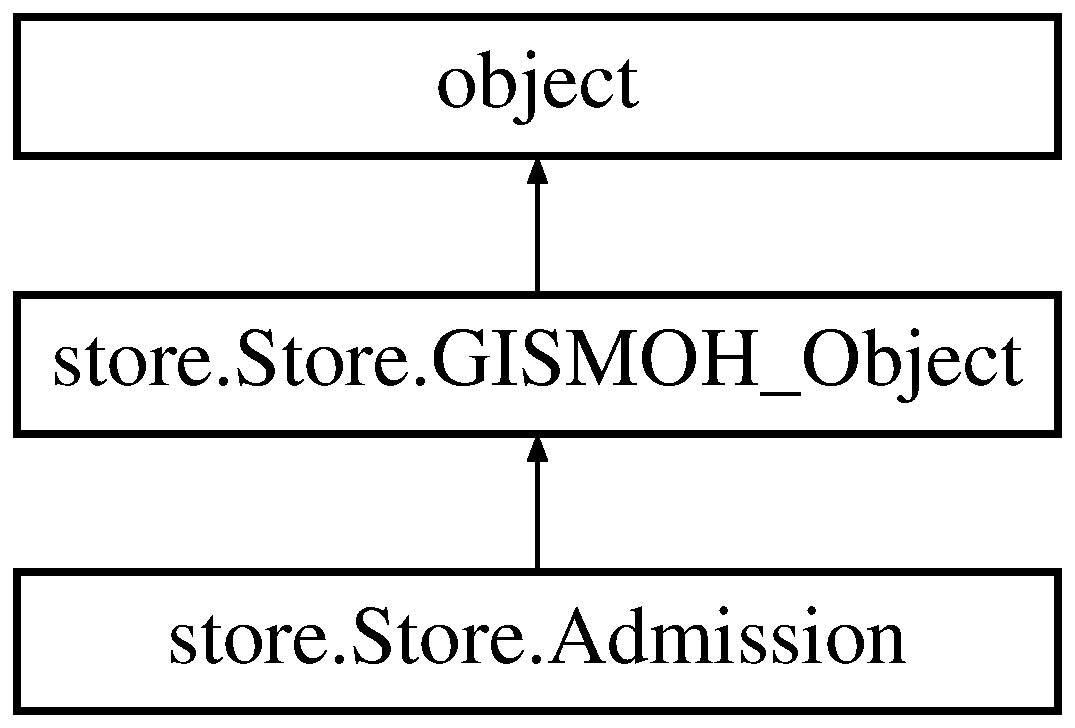
\includegraphics[height=3.000000cm]{classstore_1_1_store_1_1_admission}
\end{center}
\end{figure}
\subsection*{Public Member Functions}
\begin{DoxyCompactItemize}
\item 
\hypertarget{classstore_1_1_store_1_1_admission_a037f609d804b51df827032937ae763f5}{def {\bfseries get\-\_\-key}}\label{classstore_1_1_store_1_1_admission_a037f609d804b51df827032937ae763f5}

\item 
\hypertarget{classstore_1_1_store_1_1_admission_abf584daf4aec1336b308cad23bad1ca4}{def {\bfseries from\-\_\-dict}}\label{classstore_1_1_store_1_1_admission_abf584daf4aec1336b308cad23bad1ca4}

\end{DoxyCompactItemize}
\subsection*{Static Public Member Functions}
\begin{DoxyCompactItemize}
\item 
def \hyperlink{classstore_1_1_store_1_1_admission_a7821af99ac5ade96c0f4cb51191481d6}{get\-\_\-admissions\-\_\-at}
\begin{DoxyCompactList}\small\item\em get a list of current admissions at qry\-\_\-date \end{DoxyCompactList}\end{DoxyCompactItemize}
\subsection*{Static Public Attributes}
\begin{DoxyCompactItemize}
\item 
\hypertarget{classstore_1_1_store_1_1_admission_a0ef8ef5a0d8beb8a706f0bd5976e09cc}{{\bfseries uniq\-\_\-id} = None}\label{classstore_1_1_store_1_1_admission_a0ef8ef5a0d8beb8a706f0bd5976e09cc}

\item 
\hypertarget{classstore_1_1_store_1_1_admission_adbf8ea26eced6c5f3899d6720761f394}{{\bfseries start\-\_\-date} = None}\label{classstore_1_1_store_1_1_admission_adbf8ea26eced6c5f3899d6720761f394}

\item 
\hypertarget{classstore_1_1_store_1_1_admission_ab7d1763436a416d1f56156bfa422d76a}{{\bfseries end\-\_\-date} = None}\label{classstore_1_1_store_1_1_admission_ab7d1763436a416d1f56156bfa422d76a}

\item 
\hypertarget{classstore_1_1_store_1_1_admission_a3fae38d373802e4814a8404dfd2f5f8d}{{\bfseries patient\-\_\-id} = None}\label{classstore_1_1_store_1_1_admission_a3fae38d373802e4814a8404dfd2f5f8d}

\end{DoxyCompactItemize}


\subsection{Member Function Documentation}
\hypertarget{classstore_1_1_store_1_1_admission_a7821af99ac5ade96c0f4cb51191481d6}{\index{store\-::\-Store\-::\-Admission@{store\-::\-Store\-::\-Admission}!get\-\_\-admissions\-\_\-at@{get\-\_\-admissions\-\_\-at}}
\index{get\-\_\-admissions\-\_\-at@{get\-\_\-admissions\-\_\-at}!store::Store::Admission@{store\-::\-Store\-::\-Admission}}
\subsubsection[{get\-\_\-admissions\-\_\-at}]{\setlength{\rightskip}{0pt plus 5cm}def store.\-Store.\-Admission.\-get\-\_\-admissions\-\_\-at (
\begin{DoxyParamCaption}
\item[{}]{store, }
\item[{}]{qry\-\_\-date}
\end{DoxyParamCaption}
)\hspace{0.3cm}{\ttfamily [static]}}}\label{classstore_1_1_store_1_1_admission_a7821af99ac5ade96c0f4cb51191481d6}


get a list of current admissions at qry\-\_\-date 


\begin{DoxyParams}{Parameters}
{\em qry\-\_\-date} & \\
\hline
\end{DoxyParams}


The documentation for this class was generated from the following file\-:\begin{DoxyCompactItemize}
\item 
store/Store.\-py\end{DoxyCompactItemize}

\hypertarget{classmodules_1_1_antibiogram_1_1_antibiogram}{\section{modules.\-Antibiogram.\-Antibiogram Class Reference}
\label{classmodules_1_1_antibiogram_1_1_antibiogram}\index{modules.\-Antibiogram.\-Antibiogram@{modules.\-Antibiogram.\-Antibiogram}}
}


Takes Result objects with Antibiograms and compares them.  


Inheritance diagram for modules.\-Antibiogram.\-Antibiogram\-:\begin{figure}[H]
\begin{center}
\leavevmode
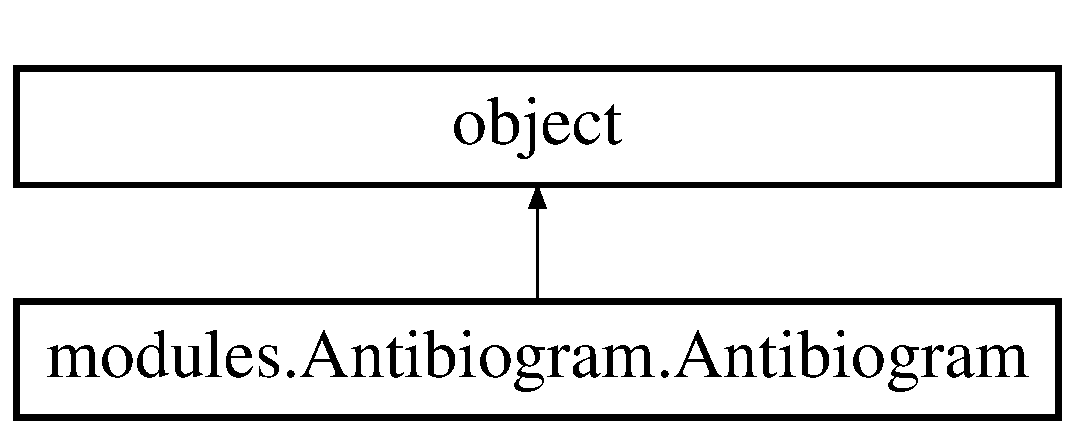
\includegraphics[height=2.000000cm]{classmodules_1_1_antibiogram_1_1_antibiogram}
\end{center}
\end{figure}
\subsection*{Public Member Functions}
\begin{DoxyCompactItemize}
\item 
\hypertarget{classmodules_1_1_antibiogram_1_1_antibiogram_a93bcdb67615825ff4ded9116df79bd68}{def {\bfseries \-\_\-\-\_\-init\-\_\-\-\_\-}}\label{classmodules_1_1_antibiogram_1_1_antibiogram_a93bcdb67615825ff4ded9116df79bd68}

\item 
def \hyperlink{classmodules_1_1_antibiogram_1_1_antibiogram_acbbd4414348d53c039eddfc40db165f8}{compare}
\begin{DoxyCompactList}\small\item\em Compare 2 antibiograms and return a similarity score. \end{DoxyCompactList}\item 
\hypertarget{classmodules_1_1_antibiogram_1_1_antibiogram_a315d6ef4e6bbfabf12f39552c5f72616}{def {\bfseries get\-\_\-nearest}}\label{classmodules_1_1_antibiogram_1_1_antibiogram_a315d6ef4e6bbfabf12f39552c5f72616}

\item 
\hypertarget{classmodules_1_1_antibiogram_1_1_antibiogram_a19e90e9a86c485f1621c4ad7e3ec5c23}{def {\bfseries get\-All\-With}}\label{classmodules_1_1_antibiogram_1_1_antibiogram_a19e90e9a86c485f1621c4ad7e3ec5c23}

\end{DoxyCompactItemize}
\subsection*{Public Attributes}
\begin{DoxyCompactItemize}
\item 
\hypertarget{classmodules_1_1_antibiogram_1_1_antibiogram_a231fc3349125734f73e1075d408aaa68}{{\bfseries store}}\label{classmodules_1_1_antibiogram_1_1_antibiogram_a231fc3349125734f73e1075d408aaa68}

\end{DoxyCompactItemize}


\subsection{Detailed Description}
Takes Result objects with Antibiograms and compares them. 

\subsection{Member Function Documentation}
\hypertarget{classmodules_1_1_antibiogram_1_1_antibiogram_acbbd4414348d53c039eddfc40db165f8}{\index{modules\-::\-Antibiogram\-::\-Antibiogram@{modules\-::\-Antibiogram\-::\-Antibiogram}!compare@{compare}}
\index{compare@{compare}!modules::Antibiogram::Antibiogram@{modules\-::\-Antibiogram\-::\-Antibiogram}}
\subsubsection[{compare}]{\setlength{\rightskip}{0pt plus 5cm}def modules.\-Antibiogram.\-Antibiogram.\-compare (
\begin{DoxyParamCaption}
\item[{}]{self, }
\item[{}]{ab1, }
\item[{}]{ab2, }
\item[{}]{mismatch\-\_\-penalty = {\ttfamily 1.0}, }
\item[{}]{gap\-\_\-penalty = {\ttfamily 0.5}}
\end{DoxyParamCaption}
)}}\label{classmodules_1_1_antibiogram_1_1_antibiogram_acbbd4414348d53c039eddfc40db165f8}


Compare 2 antibiograms and return a similarity score. 


\begin{DoxyParams}{Parameters}
{\em ab1} & Store.\-Result\-: \\
\hline
{\em ab2} & Store.\-Result\-: \\
\hline
\end{DoxyParams}


The documentation for this class was generated from the following file\-:\begin{DoxyCompactItemize}
\item 
modules/Antibiogram.\-py\end{DoxyCompactItemize}

\hypertarget{classapplication_1_1_antibiogram___test}{\section{application.\-Antibiogram\-\_\-\-Test Class Reference}
\label{classapplication_1_1_antibiogram___test}\index{application.\-Antibiogram\-\_\-\-Test@{application.\-Antibiogram\-\_\-\-Test}}
}
Inheritance diagram for application.\-Antibiogram\-\_\-\-Test\-:\begin{figure}[H]
\begin{center}
\leavevmode
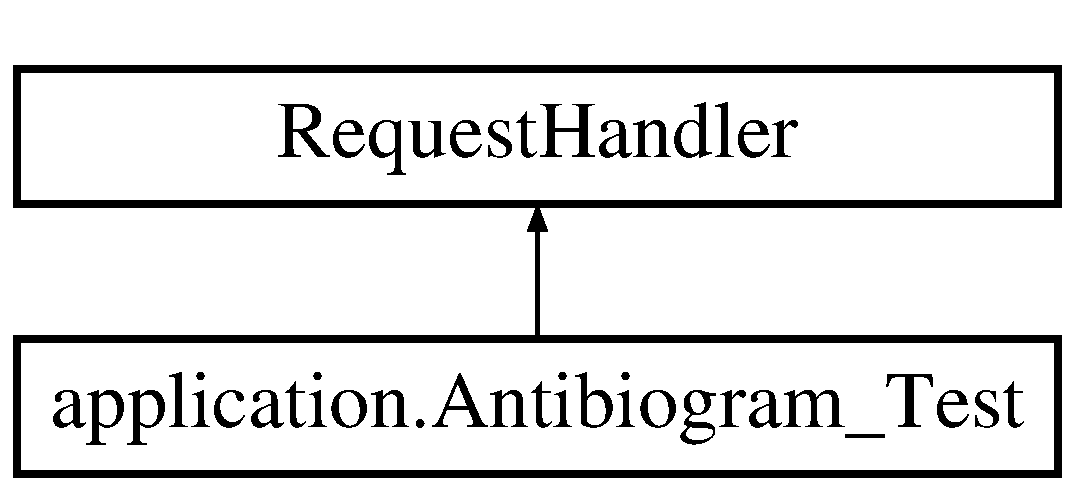
\includegraphics[height=2.000000cm]{classapplication_1_1_antibiogram___test}
\end{center}
\end{figure}
\subsection*{Public Member Functions}
\begin{DoxyCompactItemize}
\item 
\hypertarget{classapplication_1_1_antibiogram___test_a06711a7a27b3885db2353b098c18fdb2}{def {\bfseries get}}\label{classapplication_1_1_antibiogram___test_a06711a7a27b3885db2353b098c18fdb2}

\end{DoxyCompactItemize}


The documentation for this class was generated from the following file\-:\begin{DoxyCompactItemize}
\item 
application.\-py\end{DoxyCompactItemize}

\hypertarget{classtests_1_1scbu__importer_1_1_antibiogram__test}{\section{tests.\-scbu\-\_\-importer.\-Antibiogram\-\_\-test Class Reference}
\label{classtests_1_1scbu__importer_1_1_antibiogram__test}\index{tests.\-scbu\-\_\-importer.\-Antibiogram\-\_\-test@{tests.\-scbu\-\_\-importer.\-Antibiogram\-\_\-test}}
}
Inheritance diagram for tests.\-scbu\-\_\-importer.\-Antibiogram\-\_\-test\-:\begin{figure}[H]
\begin{center}
\leavevmode
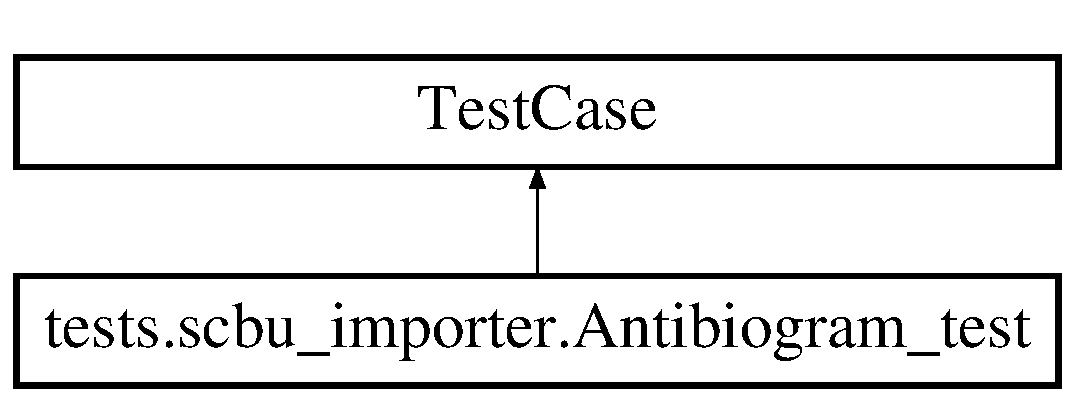
\includegraphics[height=2.000000cm]{classtests_1_1scbu__importer_1_1_antibiogram__test}
\end{center}
\end{figure}
\subsection*{Public Member Functions}
\begin{DoxyCompactItemize}
\item 
\hypertarget{classtests_1_1scbu__importer_1_1_antibiogram__test_ac8b6f6f559d9df1e6e0f5fca69b2f9da}{def {\bfseries set\-Up}}\label{classtests_1_1scbu__importer_1_1_antibiogram__test_ac8b6f6f559d9df1e6e0f5fca69b2f9da}

\item 
\hypertarget{classtests_1_1scbu__importer_1_1_antibiogram__test_a8d55b77801ec277f326a0810fc2a4acc}{def {\bfseries test\-\_\-compare\-\_\-same}}\label{classtests_1_1scbu__importer_1_1_antibiogram__test_a8d55b77801ec277f326a0810fc2a4acc}

\item 
\hypertarget{classtests_1_1scbu__importer_1_1_antibiogram__test_acbc22aa7970e0f03ff6eedb42f516453}{def {\bfseries test\-\_\-compare\-\_\-one\-\_\-diff}}\label{classtests_1_1scbu__importer_1_1_antibiogram__test_acbc22aa7970e0f03ff6eedb42f516453}

\item 
\hypertarget{classtests_1_1scbu__importer_1_1_antibiogram__test_a735cdf80ff7c090d5fc100c2db091c87}{def {\bfseries test\-\_\-compare\-\_\-one\-\_\-gap}}\label{classtests_1_1scbu__importer_1_1_antibiogram__test_a735cdf80ff7c090d5fc100c2db091c87}

\item 
\hypertarget{classtests_1_1scbu__importer_1_1_antibiogram__test_a3c8f6dc9c80ab97a1dbaf717fb22c17e}{def {\bfseries test\-\_\-compare\-\_\-two\-\_\-gap}}\label{classtests_1_1scbu__importer_1_1_antibiogram__test_a3c8f6dc9c80ab97a1dbaf717fb22c17e}

\item 
\hypertarget{classtests_1_1scbu__importer_1_1_antibiogram__test_ae106d806fa221a2a80688aea8562f7fe}{def {\bfseries test\-\_\-get\-\_\-nearest\-\_\-default}}\label{classtests_1_1scbu__importer_1_1_antibiogram__test_ae106d806fa221a2a80688aea8562f7fe}

\item 
\hypertarget{classtests_1_1scbu__importer_1_1_antibiogram__test_a73aacc613ec9096403763878f1d2f51b}{def {\bfseries test\-\_\-get\-\_\-nearest\-\_\-n}}\label{classtests_1_1scbu__importer_1_1_antibiogram__test_a73aacc613ec9096403763878f1d2f51b}

\end{DoxyCompactItemize}
\subsection*{Public Attributes}
\begin{DoxyCompactItemize}
\item 
\hypertarget{classtests_1_1scbu__importer_1_1_antibiogram__test_a5156a07f58edfa07ea7319bd87e8a0c9}{{\bfseries ab1}}\label{classtests_1_1scbu__importer_1_1_antibiogram__test_a5156a07f58edfa07ea7319bd87e8a0c9}

\end{DoxyCompactItemize}


The documentation for this class was generated from the following file\-:\begin{DoxyCompactItemize}
\item 
tests/scbu\-\_\-importer.\-py\end{DoxyCompactItemize}

\hypertarget{classstore_1_1_store_1_1_couchbase_store}{\section{store.\-Store.\-Couchbase\-Store Class Reference}
\label{classstore_1_1_store_1_1_couchbase_store}\index{store.\-Store.\-Couchbase\-Store@{store.\-Store.\-Couchbase\-Store}}
}


Connection to a database.  


\subsection*{Public Member Functions}
\begin{DoxyCompactItemize}
\item 
\hypertarget{classstore_1_1_store_1_1_couchbase_store_ab756e679cc271b5276f7f7bd39907362}{def {\bfseries \-\_\-\-\_\-init\-\_\-\-\_\-}}\label{classstore_1_1_store_1_1_couchbase_store_ab756e679cc271b5276f7f7bd39907362}

\item 
\hypertarget{classstore_1_1_store_1_1_couchbase_store_a8aea2413ee17d4f88d5d11d497c334cc}{def {\bfseries save}}\label{classstore_1_1_store_1_1_couchbase_store_a8aea2413ee17d4f88d5d11d497c334cc}

\item 
\hypertarget{classstore_1_1_store_1_1_couchbase_store_a50c6472b5c3972dff22e4662590c3ca7}{def {\bfseries fetch}}\label{classstore_1_1_store_1_1_couchbase_store_a50c6472b5c3972dff22e4662590c3ca7}

\item 
\hypertarget{classstore_1_1_store_1_1_couchbase_store_abaa51ed005860a092a94edc15c9c13ac}{def {\bfseries fetch\-\_\-objects}}\label{classstore_1_1_store_1_1_couchbase_store_abaa51ed005860a092a94edc15c9c13ac}

\item 
\hypertarget{classstore_1_1_store_1_1_couchbase_store_ae46f604d7d71ddac50f7ba27b61308a4}{def {\bfseries get\-\_\-view}}\label{classstore_1_1_store_1_1_couchbase_store_ae46f604d7d71ddac50f7ba27b61308a4}

\item 
\hypertarget{classstore_1_1_store_1_1_couchbase_store_aa23b9d3e66a1361597221b86e3ca3dad}{def {\bfseries create\-\_\-query}}\label{classstore_1_1_store_1_1_couchbase_store_aa23b9d3e66a1361597221b86e3ca3dad}

\item 
\hypertarget{classstore_1_1_store_1_1_couchbase_store_a9d6730e1dbf17f80dc120b3f3bc239c6}{def {\bfseries get\-\_\-next\-\_\-from}}\label{classstore_1_1_store_1_1_couchbase_store_a9d6730e1dbf17f80dc120b3f3bc239c6}

\item 
\hypertarget{classstore_1_1_store_1_1_couchbase_store_a7841d51ea60b77bcae3b24f5448a6a65}{def {\bfseries get\-\_\-from\-\_\-view\-\_\-by\-\_\-key}}\label{classstore_1_1_store_1_1_couchbase_store_a7841d51ea60b77bcae3b24f5448a6a65}

\end{DoxyCompactItemize}
\subsection*{Static Public Attributes}
\begin{DoxyCompactItemize}
\item 
\hypertarget{classstore_1_1_store_1_1_couchbase_store_aa5b16666e07642f870d64fcd72e17304}{{\bfseries db} = None}\label{classstore_1_1_store_1_1_couchbase_store_aa5b16666e07642f870d64fcd72e17304}

\end{DoxyCompactItemize}


\subsection{Detailed Description}
Connection to a database. 

The documentation for this class was generated from the following file\-:\begin{DoxyCompactItemize}
\item 
store/Store.\-py\end{DoxyCompactItemize}

\hypertarget{classstore_1_1_store_1_1_g_i_s_m_o_h___object}{\section{store.\-Store.\-G\-I\-S\-M\-O\-H\-\_\-\-Object Class Reference}
\label{classstore_1_1_store_1_1_g_i_s_m_o_h___object}\index{store.\-Store.\-G\-I\-S\-M\-O\-H\-\_\-\-Object@{store.\-Store.\-G\-I\-S\-M\-O\-H\-\_\-\-Object}}
}
Inheritance diagram for store.\-Store.\-G\-I\-S\-M\-O\-H\-\_\-\-Object\-:\begin{figure}[H]
\begin{center}
\leavevmode
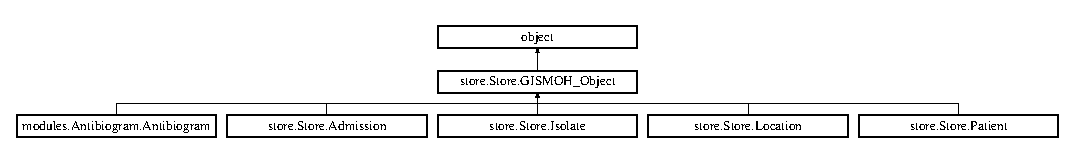
\includegraphics[height=1.866667cm]{classstore_1_1_store_1_1_g_i_s_m_o_h___object}
\end{center}
\end{figure}
\subsection*{Public Member Functions}
\begin{DoxyCompactItemize}
\item 
\hypertarget{classstore_1_1_store_1_1_g_i_s_m_o_h___object_ac3391d8ff49f41c4d90d8692fcf9ee8e}{def {\bfseries get\-\_\-key}}\label{classstore_1_1_store_1_1_g_i_s_m_o_h___object_ac3391d8ff49f41c4d90d8692fcf9ee8e}

\item 
\hypertarget{classstore_1_1_store_1_1_g_i_s_m_o_h___object_ab955e952f3fad2c1cc1909cf79bbfd25}{def {\bfseries get\-\_\-type}}\label{classstore_1_1_store_1_1_g_i_s_m_o_h___object_ab955e952f3fad2c1cc1909cf79bbfd25}

\item 
\hypertarget{classstore_1_1_store_1_1_g_i_s_m_o_h___object_a9b9e18740c48aedb2751ffbe62ca5f50}{def {\bfseries get\-\_\-dict}}\label{classstore_1_1_store_1_1_g_i_s_m_o_h___object_a9b9e18740c48aedb2751ffbe62ca5f50}

\item 
\hypertarget{classstore_1_1_store_1_1_g_i_s_m_o_h___object_a2e3683c267f623cd7740c7f47da42880}{def {\bfseries from\-\_\-dict}}\label{classstore_1_1_store_1_1_g_i_s_m_o_h___object_a2e3683c267f623cd7740c7f47da42880}

\end{DoxyCompactItemize}


The documentation for this class was generated from the following file\-:\begin{DoxyCompactItemize}
\item 
store/Store.\-py\end{DoxyCompactItemize}

\hypertarget{classstore_1_1_store_1_1_isolate}{\section{store.\-Store.\-Isolate Class Reference}
\label{classstore_1_1_store_1_1_isolate}\index{store.\-Store.\-Isolate@{store.\-Store.\-Isolate}}
}
Inheritance diagram for store.\-Store.\-Isolate\-:\begin{figure}[H]
\begin{center}
\leavevmode
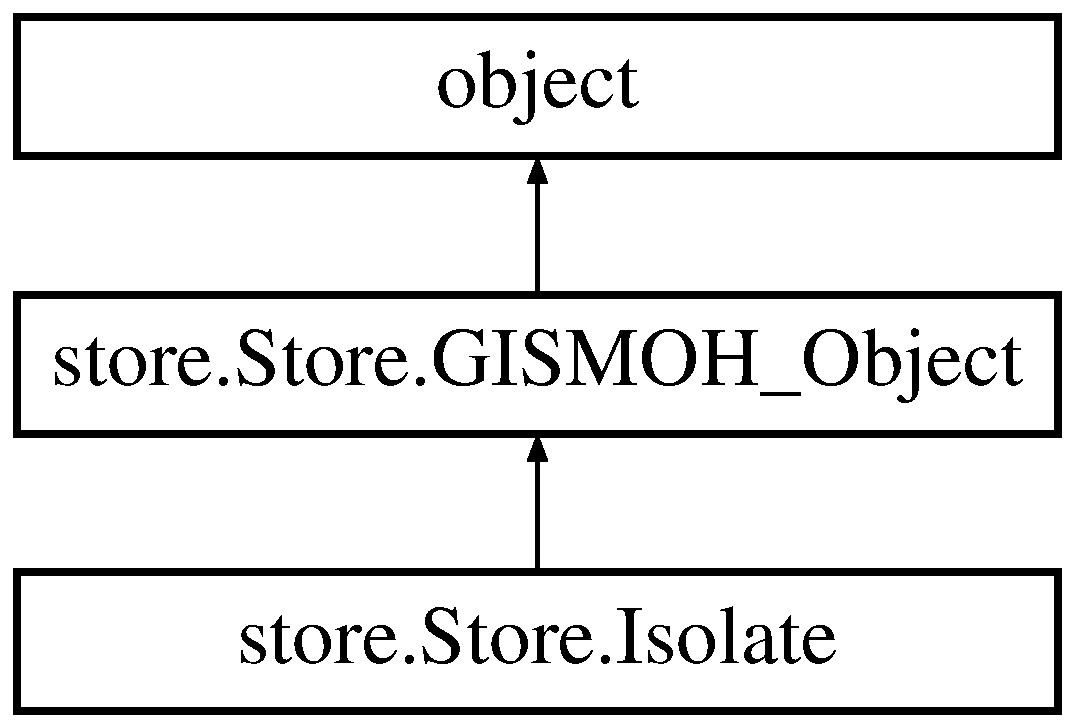
\includegraphics[height=3.000000cm]{classstore_1_1_store_1_1_isolate}
\end{center}
\end{figure}
\subsection*{Public Member Functions}
\begin{DoxyCompactItemize}
\item 
\hypertarget{classstore_1_1_store_1_1_isolate_a5c16cc9d4271954b3ac7b15a1825e282}{def {\bfseries get\-\_\-key}}\label{classstore_1_1_store_1_1_isolate_a5c16cc9d4271954b3ac7b15a1825e282}

\item 
\hypertarget{classstore_1_1_store_1_1_isolate_ac1731fe05dad361255acb32bd5709041}{def {\bfseries from\-\_\-dict}}\label{classstore_1_1_store_1_1_isolate_ac1731fe05dad361255acb32bd5709041}

\end{DoxyCompactItemize}
\subsection*{Static Public Member Functions}
\begin{DoxyCompactItemize}
\item 
\hypertarget{classstore_1_1_store_1_1_isolate_abb9b3cf89c61fccfe95d5ec2aa13e962}{def {\bfseries get\-\_\-isolates\-\_\-taken\-\_\-between}}\label{classstore_1_1_store_1_1_isolate_abb9b3cf89c61fccfe95d5ec2aa13e962}

\end{DoxyCompactItemize}
\subsection*{Static Public Attributes}
\begin{DoxyCompactItemize}
\item 
\hypertarget{classstore_1_1_store_1_1_isolate_ab6c42ec02ecd9a44732058c4aae265c9}{{\bfseries lab\-\_\-number} = None}\label{classstore_1_1_store_1_1_isolate_ab6c42ec02ecd9a44732058c4aae265c9}

\item 
\hypertarget{classstore_1_1_store_1_1_isolate_ae75afdb7ee3b0064c954d04137a780e8}{{\bfseries patient\-\_\-id} = None}\label{classstore_1_1_store_1_1_isolate_ae75afdb7ee3b0064c954d04137a780e8}

\item 
\hypertarget{classstore_1_1_store_1_1_isolate_aeb1865270e2f3c91a369dfe3ee623e48}{{\bfseries date\-\_\-taken} = None}\label{classstore_1_1_store_1_1_isolate_aeb1865270e2f3c91a369dfe3ee623e48}

\item 
\hypertarget{classstore_1_1_store_1_1_isolate_adc178450407285b305d7e5cecc5f3c18}{{\bfseries organism} = None}\label{classstore_1_1_store_1_1_isolate_adc178450407285b305d7e5cecc5f3c18}

\item 
\hypertarget{classstore_1_1_store_1_1_isolate_a6e37fe0a9078265740a69500412c5f22}{{\bfseries sample\-\_\-site} = None}\label{classstore_1_1_store_1_1_isolate_a6e37fe0a9078265740a69500412c5f22}

\item 
\hypertarget{classstore_1_1_store_1_1_isolate_accd39029d15f572cf5b0df8e172a30da}{{\bfseries location} = None}\label{classstore_1_1_store_1_1_isolate_accd39029d15f572cf5b0df8e172a30da}

\item 
\hypertarget{classstore_1_1_store_1_1_isolate_a6da2aeb5cc045213fc76e2118c68ac98}{{\bfseries genotypic\-\_\-resistance} = None}\label{classstore_1_1_store_1_1_isolate_a6da2aeb5cc045213fc76e2118c68ac98}

\item 
\hypertarget{classstore_1_1_store_1_1_isolate_a70dbfa8aa91dfc5817dfdfe54f879b5d}{{\bfseries phenotypic\-\_\-resistance} = None}\label{classstore_1_1_store_1_1_isolate_a70dbfa8aa91dfc5817dfdfe54f879b5d}

\end{DoxyCompactItemize}


The documentation for this class was generated from the following file\-:\begin{DoxyCompactItemize}
\item 
store/Store.\-py\end{DoxyCompactItemize}

\hypertarget{classapplication_1_1_isolates}{\section{application.\-Isolates Class Reference}
\label{classapplication_1_1_isolates}\index{application.\-Isolates@{application.\-Isolates}}
}
Inheritance diagram for application.\-Isolates\-:\begin{figure}[H]
\begin{center}
\leavevmode
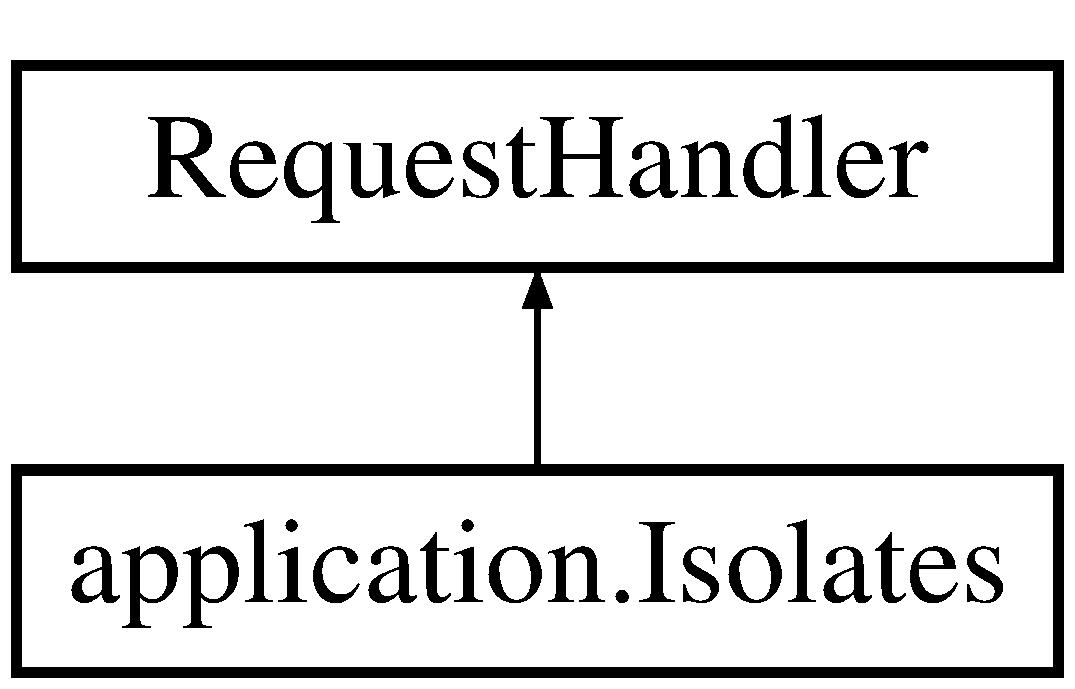
\includegraphics[height=2.000000cm]{classapplication_1_1_isolates}
\end{center}
\end{figure}
\subsection*{Public Member Functions}
\begin{DoxyCompactItemize}
\item 
\hypertarget{classapplication_1_1_isolates_ad771bde1f560d14e70fe9e970bd491d3}{def {\bfseries get}}\label{classapplication_1_1_isolates_ad771bde1f560d14e70fe9e970bd491d3}

\end{DoxyCompactItemize}


The documentation for this class was generated from the following file\-:\begin{DoxyCompactItemize}
\item 
application.\-py\end{DoxyCompactItemize}

\hypertarget{classstore_1_1_store_1_1_location}{\section{store.\-Store.\-Location Class Reference}
\label{classstore_1_1_store_1_1_location}\index{store.\-Store.\-Location@{store.\-Store.\-Location}}
}
Inheritance diagram for store.\-Store.\-Location\-:\begin{figure}[H]
\begin{center}
\leavevmode
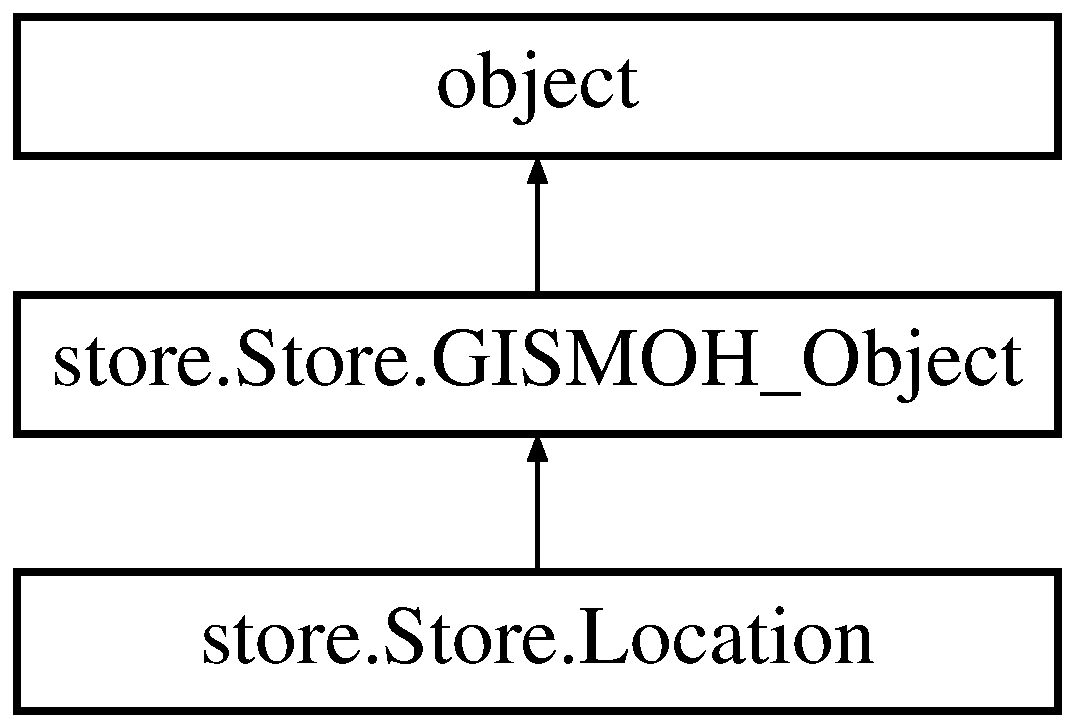
\includegraphics[height=3.000000cm]{classstore_1_1_store_1_1_location}
\end{center}
\end{figure}
\subsection*{Static Public Attributes}
\begin{DoxyCompactItemize}
\item 
\hypertarget{classstore_1_1_store_1_1_location_a4f7384df1dac7954a4b47ddb5f73e547}{{\bfseries ward} = None}\label{classstore_1_1_store_1_1_location_a4f7384df1dac7954a4b47ddb5f73e547}

\item 
\hypertarget{classstore_1_1_store_1_1_location_ae81364ac93cb4db0b016c3d514439e00}{{\bfseries arrived} = None}\label{classstore_1_1_store_1_1_location_ae81364ac93cb4db0b016c3d514439e00}

\item 
\hypertarget{classstore_1_1_store_1_1_location_a8faaea31d4b72ea58051f323ccee5937}{{\bfseries left} = None}\label{classstore_1_1_store_1_1_location_a8faaea31d4b72ea58051f323ccee5937}

\end{DoxyCompactItemize}
\subsection*{Additional Inherited Members}


The documentation for this class was generated from the following file\-:\begin{DoxyCompactItemize}
\item 
store/Store.\-py\end{DoxyCompactItemize}

\hypertarget{classtests_1_1_location__if_1_1_location_i_f_tests}{\section{tests.\-Location\-\_\-if.\-Location\-I\-F\-Tests Class Reference}
\label{classtests_1_1_location__if_1_1_location_i_f_tests}\index{tests.\-Location\-\_\-if.\-Location\-I\-F\-Tests@{tests.\-Location\-\_\-if.\-Location\-I\-F\-Tests}}
}
Inheritance diagram for tests.\-Location\-\_\-if.\-Location\-I\-F\-Tests\-:\begin{figure}[H]
\begin{center}
\leavevmode
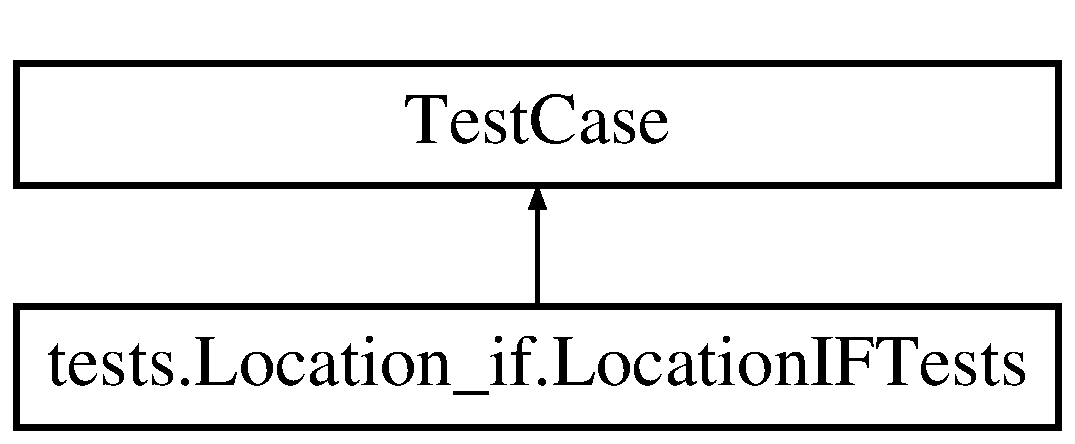
\includegraphics[height=2.000000cm]{classtests_1_1_location__if_1_1_location_i_f_tests}
\end{center}
\end{figure}
\subsection*{Public Member Functions}
\begin{DoxyCompactItemize}
\item 
\hypertarget{classtests_1_1_location__if_1_1_location_i_f_tests_ad056fc5b8cc9e805738ab45a695ca323}{def {\bfseries set\-Up}}\label{classtests_1_1_location__if_1_1_location_i_f_tests_ad056fc5b8cc9e805738ab45a695ca323}

\item 
\hypertarget{classtests_1_1_location__if_1_1_location_i_f_tests_a5f193b8d207f01725bb382b9d4fce667}{def {\bfseries test\-\_\-get\-\_\-by\-\_\-id}}\label{classtests_1_1_location__if_1_1_location_i_f_tests_a5f193b8d207f01725bb382b9d4fce667}

\item 
\hypertarget{classtests_1_1_location__if_1_1_location_i_f_tests_a9aa54e0a42d00be055e32f3dd9b03a21}{def {\bfseries test\-\_\-get\-\_\-overlaps}}\label{classtests_1_1_location__if_1_1_location_i_f_tests_a9aa54e0a42d00be055e32f3dd9b03a21}

\item 
\hypertarget{classtests_1_1_location__if_1_1_location_i_f_tests_a3e233c3a2001ccbc455ea9732e7c61cc}{def {\bfseries test\-\_\-overlaps\-\_\-length}}\label{classtests_1_1_location__if_1_1_location_i_f_tests_a3e233c3a2001ccbc455ea9732e7c61cc}

\item 
\hypertarget{classtests_1_1_location__if_1_1_location_i_f_tests_a1dc450a9309495c6007c055a21288da0}{def {\bfseries test\-\_\-get\-\_\-location\-\_\-at\-\_\-date}}\label{classtests_1_1_location__if_1_1_location_i_f_tests_a1dc450a9309495c6007c055a21288da0}

\item 
\hypertarget{classtests_1_1_location__if_1_1_location_i_f_tests_a04e8e3a28c07d32cf031a94a4ae6847f}{def {\bfseries test\-\_\-get\-\_\-admission\-\_\-at\-\_\-date}}\label{classtests_1_1_location__if_1_1_location_i_f_tests_a04e8e3a28c07d32cf031a94a4ae6847f}

\end{DoxyCompactItemize}
\subsection*{Public Attributes}
\begin{DoxyCompactItemize}
\item 
\hypertarget{classtests_1_1_location__if_1_1_location_i_f_tests_ac10603a5576a6a6ae5c3df1b4a2f067e}{{\bfseries con}}\label{classtests_1_1_location__if_1_1_location_i_f_tests_ac10603a5576a6a6ae5c3df1b4a2f067e}

\end{DoxyCompactItemize}


The documentation for this class was generated from the following file\-:\begin{DoxyCompactItemize}
\item 
tests/Location\-\_\-if.\-py\end{DoxyCompactItemize}

\hypertarget{classmodules_1_1_location_1_1_location_interface}{\section{modules.\-Location.\-Location\-Interface Class Reference}
\label{classmodules_1_1_location_1_1_location_interface}\index{modules.\-Location.\-Location\-Interface@{modules.\-Location.\-Location\-Interface}}
}
Inheritance diagram for modules.\-Location.\-Location\-Interface\-:\begin{figure}[H]
\begin{center}
\leavevmode
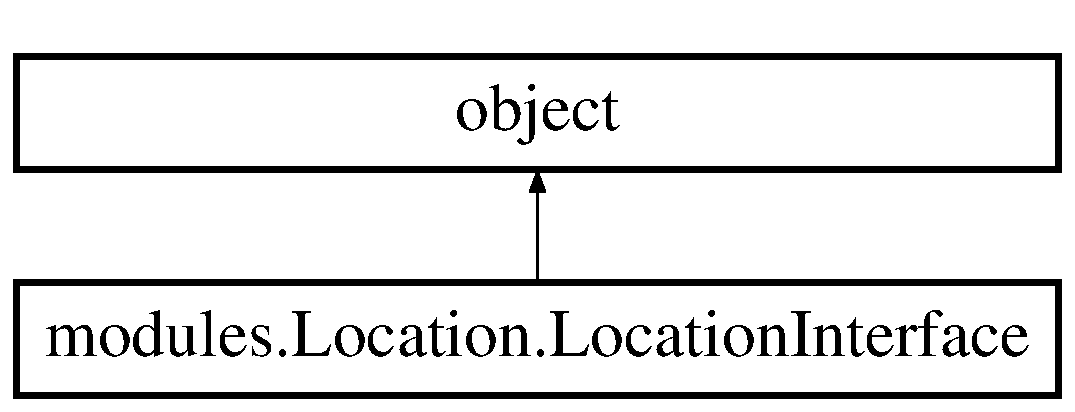
\includegraphics[height=2.000000cm]{classmodules_1_1_location_1_1_location_interface}
\end{center}
\end{figure}
\subsection*{Public Member Functions}
\begin{DoxyCompactItemize}
\item 
\hypertarget{classmodules_1_1_location_1_1_location_interface_a2471fcaae71fa16c1e8221279c690f3d}{def {\bfseries \-\_\-\-\_\-init\-\_\-\-\_\-}}\label{classmodules_1_1_location_1_1_location_interface_a2471fcaae71fa16c1e8221279c690f3d}

\item 
def \hyperlink{classmodules_1_1_location_1_1_location_interface_ab9bdfdc0a0595ecd79e680bf37beb87d}{get\-\_\-overlaps\-\_\-with\-\_\-location}
\begin{DoxyCompactList}\small\item\em Get overlaps with a location. \end{DoxyCompactList}\item 
\hypertarget{classmodules_1_1_location_1_1_location_interface_a6ee9111bccd8d5fbf747450799a1d25e}{def {\bfseries get\-\_\-overlaps\-\_\-with\-\_\-patient}}\label{classmodules_1_1_location_1_1_location_interface_a6ee9111bccd8d5fbf747450799a1d25e}

\end{DoxyCompactItemize}
\subsection*{Public Attributes}
\begin{DoxyCompactItemize}
\item 
\hypertarget{classmodules_1_1_location_1_1_location_interface_a756e94a9b2492c21bb92de0fdfbb2eb6}{{\bfseries store}}\label{classmodules_1_1_location_1_1_location_interface_a756e94a9b2492c21bb92de0fdfbb2eb6}

\end{DoxyCompactItemize}


\subsection{Member Function Documentation}
\hypertarget{classmodules_1_1_location_1_1_location_interface_ab9bdfdc0a0595ecd79e680bf37beb87d}{\index{modules\-::\-Location\-::\-Location\-Interface@{modules\-::\-Location\-::\-Location\-Interface}!get\-\_\-overlaps\-\_\-with\-\_\-location@{get\-\_\-overlaps\-\_\-with\-\_\-location}}
\index{get\-\_\-overlaps\-\_\-with\-\_\-location@{get\-\_\-overlaps\-\_\-with\-\_\-location}!modules::Location::LocationInterface@{modules\-::\-Location\-::\-Location\-Interface}}
\subsubsection[{get\-\_\-overlaps\-\_\-with\-\_\-location}]{\setlength{\rightskip}{0pt plus 5cm}def modules.\-Location.\-Location\-Interface.\-get\-\_\-overlaps\-\_\-with\-\_\-location (
\begin{DoxyParamCaption}
\item[{}]{self, }
\item[{}]{location}
\end{DoxyParamCaption}
)}}\label{classmodules_1_1_location_1_1_location_interface_ab9bdfdc0a0595ecd79e680bf37beb87d}


Get overlaps with a location. 


\begin{DoxyParams}{Parameters}
{\em location} & Store.\-Location\-: \\
\hline
\end{DoxyParams}


The documentation for this class was generated from the following file\-:\begin{DoxyCompactItemize}
\item 
modules/Location.\-py\end{DoxyCompactItemize}

\hypertarget{classapplication_1_1_locations}{\section{application.\-Locations Class Reference}
\label{classapplication_1_1_locations}\index{application.\-Locations@{application.\-Locations}}
}
Inheritance diagram for application.\-Locations\-:\begin{figure}[H]
\begin{center}
\leavevmode
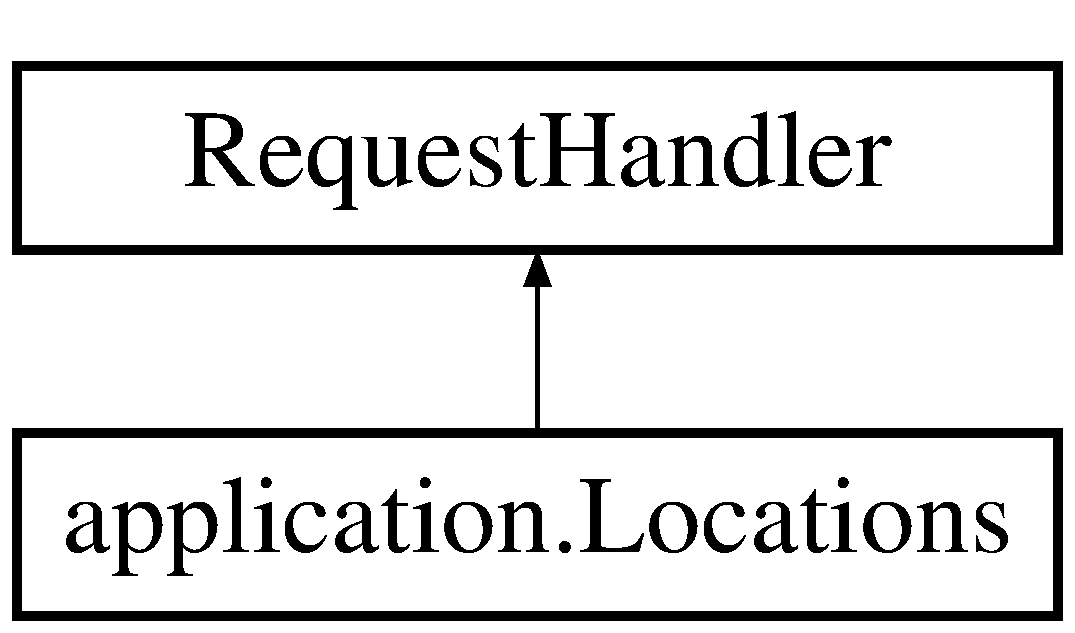
\includegraphics[height=2.000000cm]{classapplication_1_1_locations}
\end{center}
\end{figure}
\subsection*{Public Member Functions}
\begin{DoxyCompactItemize}
\item 
\hypertarget{classapplication_1_1_locations_a64006805003a30f3ca7b4c15481fa18a}{def {\bfseries get}}\label{classapplication_1_1_locations_a64006805003a30f3ca7b4c15481fa18a}

\end{DoxyCompactItemize}


The documentation for this class was generated from the following file\-:\begin{DoxyCompactItemize}
\item 
application.\-py\end{DoxyCompactItemize}

\hypertarget{classtests_1_1all_1_1main__test}{\section{tests.\-all.\-main\-\_\-test Class Reference}
\label{classtests_1_1all_1_1main__test}\index{tests.\-all.\-main\-\_\-test@{tests.\-all.\-main\-\_\-test}}
}
Inheritance diagram for tests.\-all.\-main\-\_\-test\-:\begin{figure}[H]
\begin{center}
\leavevmode
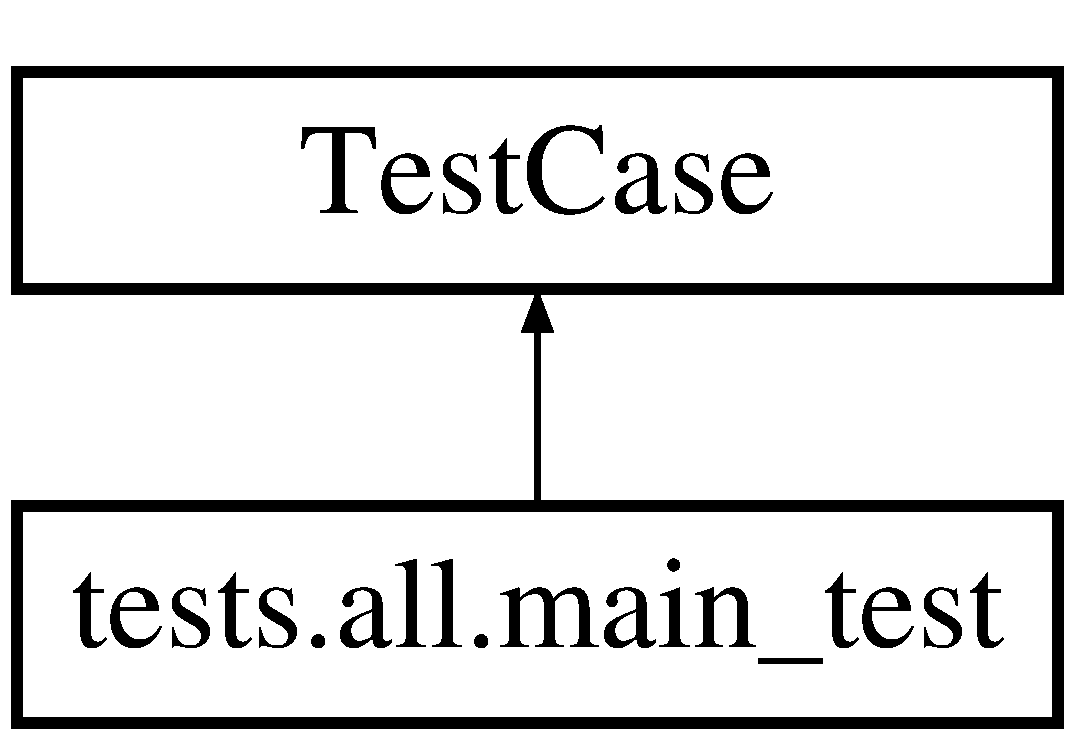
\includegraphics[height=2.000000cm]{classtests_1_1all_1_1main__test}
\end{center}
\end{figure}
\subsection*{Public Member Functions}
\begin{DoxyCompactItemize}
\item 
\hypertarget{classtests_1_1all_1_1main__test_a52658a6f5c9860fee1eee9eb6bd276f7}{def {\bfseries test\-\_\-connect}}\label{classtests_1_1all_1_1main__test_a52658a6f5c9860fee1eee9eb6bd276f7}

\item 
\hypertarget{classtests_1_1all_1_1main__test_a81358c42b298ceccfa01e84e40aad061}{def {\bfseries test\-\_\-bad\-\_\-bucket}}\label{classtests_1_1all_1_1main__test_a81358c42b298ceccfa01e84e40aad061}

\item 
\hypertarget{classtests_1_1all_1_1main__test_a3d51827c15fd6f7fffbfc6ade785d64f}{def {\bfseries test\-\_\-auth\-\_\-fail}}\label{classtests_1_1all_1_1main__test_a3d51827c15fd6f7fffbfc6ade785d64f}

\item 
\hypertarget{classtests_1_1all_1_1main__test_a91c8b72555ef67a9349e1e91ed74ccd3}{def {\bfseries test\-\_\-format\-\_\-nhs\-\_\-number}}\label{classtests_1_1all_1_1main__test_a91c8b72555ef67a9349e1e91ed74ccd3}

\item 
\hypertarget{classtests_1_1all_1_1main__test_aefe6fcb2fde732d4ec6afdd460fcd91b}{def {\bfseries test\-\_\-validate\-\_\-nhs\-\_\-number\-\_\-bad}}\label{classtests_1_1all_1_1main__test_aefe6fcb2fde732d4ec6afdd460fcd91b}

\item 
\hypertarget{classtests_1_1all_1_1main__test_ac6a09a4869b4cab663e8716e78e06d3c}{def {\bfseries test\-\_\-validate\-\_\-nhs\-\_\-number\-\_\-good}}\label{classtests_1_1all_1_1main__test_ac6a09a4869b4cab663e8716e78e06d3c}

\item 
\hypertarget{classtests_1_1all_1_1main__test_af5c62265a618165f87b4dc28d153ea7d}{def {\bfseries test\-\_\-add\-\_\-patientself}}\label{classtests_1_1all_1_1main__test_af5c62265a618165f87b4dc28d153ea7d}

\item 
\hypertarget{classtests_1_1all_1_1main__test_a6880211736510e2c82fb0c0f2796e339}{def {\bfseries test\-\_\-add\-\_\-patient2}}\label{classtests_1_1all_1_1main__test_a6880211736510e2c82fb0c0f2796e339}

\item 
\hypertarget{classtests_1_1all_1_1main__test_a9f35cb8ae69eb78360f991e5e3245945}{def {\bfseries test\-\_\-get\-\_\-patientself}}\label{classtests_1_1all_1_1main__test_a9f35cb8ae69eb78360f991e5e3245945}

\item 
\hypertarget{classtests_1_1all_1_1main__test_a544c867960638ac4be4302b6b968a1f4}{def {\bfseries test\-\_\-get\-\_\-patients}}\label{classtests_1_1all_1_1main__test_a544c867960638ac4be4302b6b968a1f4}

\item 
\hypertarget{classtests_1_1all_1_1main__test_a9f35cb8ae69eb78360f991e5e3245945}{def {\bfseries test\-\_\-get\-\_\-patientself}}\label{classtests_1_1all_1_1main__test_a9f35cb8ae69eb78360f991e5e3245945}

\item 
\hypertarget{classtests_1_1all_1_1main__test_af6a0e92e31ffa992c0466de2046709f0}{def {\bfseries test\-\_\-from\-\_\-dict\-\_\-nomap}}\label{classtests_1_1all_1_1main__test_af6a0e92e31ffa992c0466de2046709f0}

\item 
\hypertarget{classtests_1_1all_1_1main__test_af6a0e92e31ffa992c0466de2046709f0}{def {\bfseries test\-\_\-from\-\_\-dict\-\_\-nomap}}\label{classtests_1_1all_1_1main__test_af6a0e92e31ffa992c0466de2046709f0}

\item 
\hypertarget{classtests_1_1all_1_1main__test_ad1c1d8e93fc850e4919598f97e0bf4b6}{def {\bfseries test\-\_\-bad\-\_\-get\-\_\-key}}\label{classtests_1_1all_1_1main__test_ad1c1d8e93fc850e4919598f97e0bf4b6}

\end{DoxyCompactItemize}
\subsection*{Static Public Attributes}
\begin{DoxyCompactItemize}
\item 
\hypertarget{classtests_1_1all_1_1main__test_a57fb15f006c62f0e6107b550ff0cfc37}{{\bfseries con} = None}\label{classtests_1_1all_1_1main__test_a57fb15f006c62f0e6107b550ff0cfc37}

\end{DoxyCompactItemize}


The documentation for this class was generated from the following file\-:\begin{DoxyCompactItemize}
\item 
tests/all.\-py\end{DoxyCompactItemize}

\hypertarget{classapplication_1_1_main_handler}{\section{application.\-Main\-Handler Class Reference}
\label{classapplication_1_1_main_handler}\index{application.\-Main\-Handler@{application.\-Main\-Handler}}
}


Index page handler.  


Inheritance diagram for application.\-Main\-Handler\-:\begin{figure}[H]
\begin{center}
\leavevmode
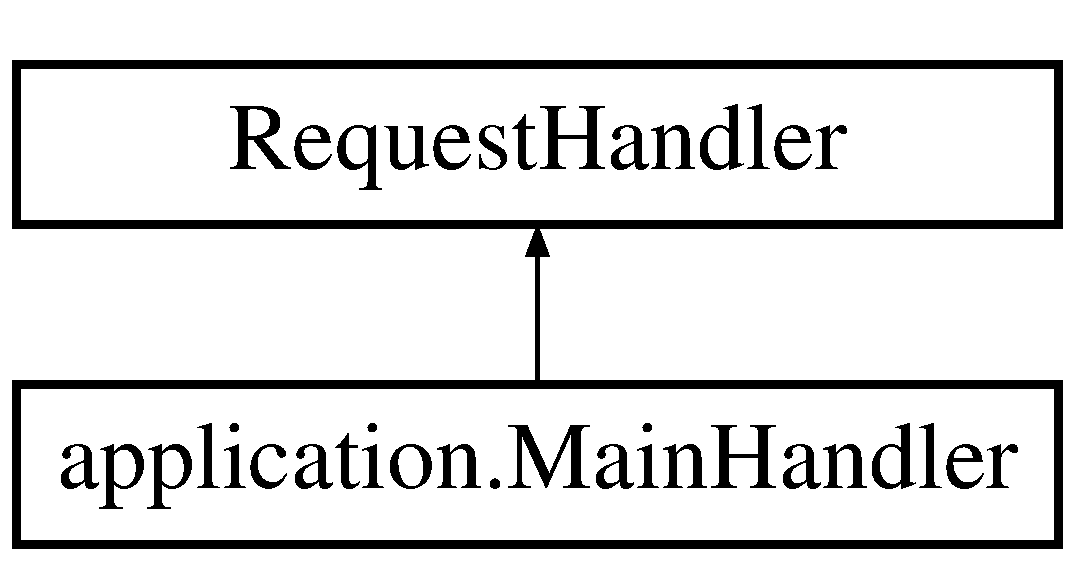
\includegraphics[height=2.000000cm]{classapplication_1_1_main_handler}
\end{center}
\end{figure}
\subsection*{Public Member Functions}
\begin{DoxyCompactItemize}
\item 
\hypertarget{classapplication_1_1_main_handler_ae71c755ef5ff2ae9b026ebdbaf60ea69}{def {\bfseries get}}\label{classapplication_1_1_main_handler_ae71c755ef5ff2ae9b026ebdbaf60ea69}

\end{DoxyCompactItemize}


\subsection{Detailed Description}
Index page handler. 

The documentation for this class was generated from the following file\-:\begin{DoxyCompactItemize}
\item 
application.\-py\end{DoxyCompactItemize}

\hypertarget{classutils_1_1_modulus11_1_1_mod11}{\section{utils.\-Modulus11.\-Mod11 Class Reference}
\label{classutils_1_1_modulus11_1_1_mod11}\index{utils.\-Modulus11.\-Mod11@{utils.\-Modulus11.\-Mod11}}
}
\subsection*{Static Public Member Functions}
\begin{DoxyCompactItemize}
\item 
\hypertarget{classutils_1_1_modulus11_1_1_mod11_a883c6c7706e04d73af197fa6c23e7e22}{def {\bfseries calculate}}\label{classutils_1_1_modulus11_1_1_mod11_a883c6c7706e04d73af197fa6c23e7e22}

\item 
\hypertarget{classutils_1_1_modulus11_1_1_mod11_afeea820d568b05a3d22dc274cdd32b7f}{def {\bfseries check}}\label{classutils_1_1_modulus11_1_1_mod11_afeea820d568b05a3d22dc274cdd32b7f}

\end{DoxyCompactItemize}


The documentation for this class was generated from the following file\-:\begin{DoxyCompactItemize}
\item 
utils/Modulus11.\-py\end{DoxyCompactItemize}

\hypertarget{classstore_1_1_store_1_1_m_s_s_q_l_store}{\section{store.\-Store.\-M\-S\-S\-Q\-L\-Store Class Reference}
\label{classstore_1_1_store_1_1_m_s_s_q_l_store}\index{store.\-Store.\-M\-S\-S\-Q\-L\-Store@{store.\-Store.\-M\-S\-S\-Q\-L\-Store}}
}
\subsection*{Public Member Functions}
\begin{DoxyCompactItemize}
\item 
\hypertarget{classstore_1_1_store_1_1_m_s_s_q_l_store_a936a83c64dbcfc6429f0ca518ea1b4a3}{def {\bfseries \-\_\-\-\_\-init\-\_\-\-\_\-}}\label{classstore_1_1_store_1_1_m_s_s_q_l_store_a936a83c64dbcfc6429f0ca518ea1b4a3}

\end{DoxyCompactItemize}
\subsection*{Static Public Attributes}
\begin{DoxyCompactItemize}
\item 
\hypertarget{classstore_1_1_store_1_1_m_s_s_q_l_store_adac08648d219367b39d399c0f6c82cb8}{{\bfseries db} = None}\label{classstore_1_1_store_1_1_m_s_s_q_l_store_adac08648d219367b39d399c0f6c82cb8}

\end{DoxyCompactItemize}


The documentation for this class was generated from the following file\-:\begin{DoxyCompactItemize}
\item 
store/Store.\-py\end{DoxyCompactItemize}

\hypertarget{classapplication_1_1_overlap_handler}{\section{application.\-Overlap\-Handler Class Reference}
\label{classapplication_1_1_overlap_handler}\index{application.\-Overlap\-Handler@{application.\-Overlap\-Handler}}
}
Inheritance diagram for application.\-Overlap\-Handler\-:\begin{figure}[H]
\begin{center}
\leavevmode
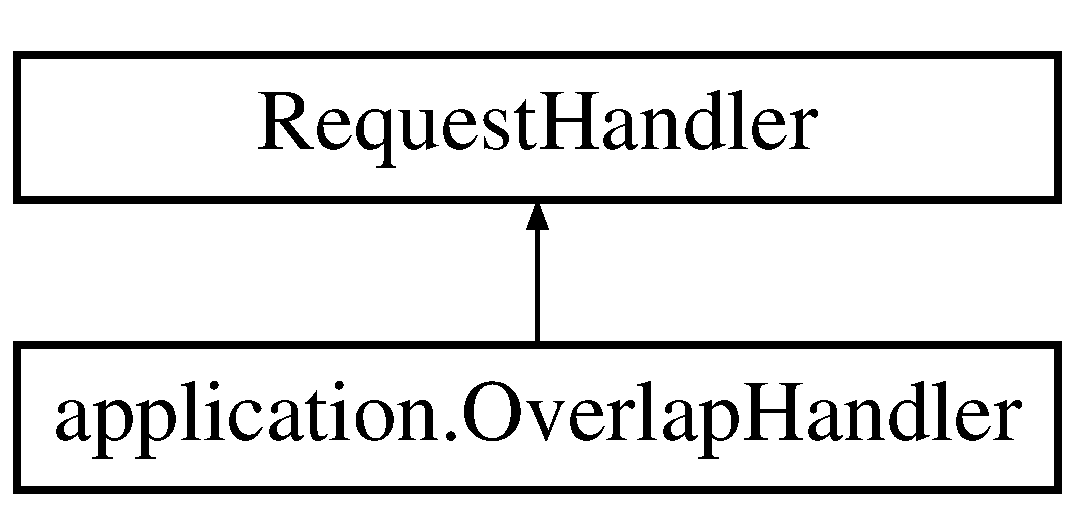
\includegraphics[height=2.000000cm]{classapplication_1_1_overlap_handler}
\end{center}
\end{figure}
\subsection*{Public Member Functions}
\begin{DoxyCompactItemize}
\item 
\hypertarget{classapplication_1_1_overlap_handler_a67ccb08d9c3d516e7d97af9025032e6b}{def {\bfseries get}}\label{classapplication_1_1_overlap_handler_a67ccb08d9c3d516e7d97af9025032e6b}

\end{DoxyCompactItemize}


The documentation for this class was generated from the following file\-:\begin{DoxyCompactItemize}
\item 
application.\-py\end{DoxyCompactItemize}

\hypertarget{classstore_1_1_store_1_1_patient}{\section{store.\-Store.\-Patient Class Reference}
\label{classstore_1_1_store_1_1_patient}\index{store.\-Store.\-Patient@{store.\-Store.\-Patient}}
}
Inheritance diagram for store.\-Store.\-Patient\-:\begin{figure}[H]
\begin{center}
\leavevmode
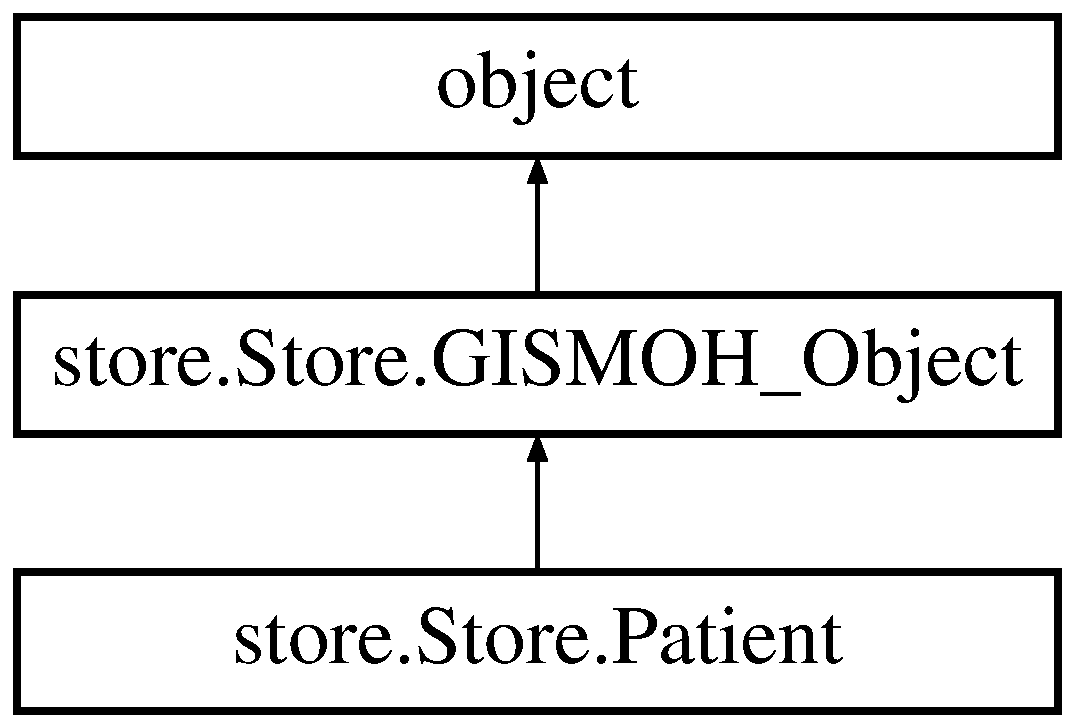
\includegraphics[height=3.000000cm]{classstore_1_1_store_1_1_patient}
\end{center}
\end{figure}
\subsection*{Public Member Functions}
\begin{DoxyCompactItemize}
\item 
\hypertarget{classstore_1_1_store_1_1_patient_ac8a2ecab27100f33c75fafa247298a97}{def {\bfseries \-\_\-\-\_\-init\-\_\-\-\_\-}}\label{classstore_1_1_store_1_1_patient_ac8a2ecab27100f33c75fafa247298a97}

\item 
\hypertarget{classstore_1_1_store_1_1_patient_a4dbaa068f510cf2686036a1fffc91fa9}{def {\bfseries get\-\_\-key\-\_\-field}}\label{classstore_1_1_store_1_1_patient_a4dbaa068f510cf2686036a1fffc91fa9}

\item 
\hypertarget{classstore_1_1_store_1_1_patient_a89d5fd5b6852bfd5efd4113ad12be491}{def \hyperlink{classstore_1_1_store_1_1_patient_a89d5fd5b6852bfd5efd4113ad12be491}{get\-\_\-key}}\label{classstore_1_1_store_1_1_patient_a89d5fd5b6852bfd5efd4113ad12be491}

\begin{DoxyCompactList}\small\item\em return the anonymised unique identifier of the \hyperlink{classstore_1_1_store_1_1_patient}{Patient} \end{DoxyCompactList}\item 
\hypertarget{classstore_1_1_store_1_1_patient_a44c7f2261c5c26138f88b1931d80b965}{def {\bfseries from\-\_\-dict}}\label{classstore_1_1_store_1_1_patient_a44c7f2261c5c26138f88b1931d80b965}

\end{DoxyCompactItemize}
\subsection*{Static Public Member Functions}
\begin{DoxyCompactItemize}
\item 
\hypertarget{classstore_1_1_store_1_1_patient_ab4c7a67cbca4e6810a537964a88fd326}{def \hyperlink{classstore_1_1_store_1_1_patient_ab4c7a67cbca4e6810a537964a88fd326}{format\-\_\-nhs\-\_\-number}}\label{classstore_1_1_store_1_1_patient_ab4c7a67cbca4e6810a537964a88fd326}

\begin{DoxyCompactList}\small\item\em Get N\-H\-S Number in a the format 000-\/000-\/0000. \end{DoxyCompactList}\item 
\hypertarget{classstore_1_1_store_1_1_patient_a33925c8fd37fcda8394f2fc819b4c397}{def {\bfseries validate\-\_\-nhs\-\_\-number}}\label{classstore_1_1_store_1_1_patient_a33925c8fd37fcda8394f2fc819b4c397}

\end{DoxyCompactItemize}
\subsection*{Static Public Attributes}
\begin{DoxyCompactItemize}
\item 
\hypertarget{classstore_1_1_store_1_1_patient_a7ce52748fe80fbdd12ebb3ce4b880d28}{\hyperlink{classstore_1_1_store_1_1_patient_a7ce52748fe80fbdd12ebb3ce4b880d28}{uniq\-\_\-id} = None}\label{classstore_1_1_store_1_1_patient_a7ce52748fe80fbdd12ebb3ce4b880d28}

\begin{DoxyCompactList}\small\item\em internal G\-I\-S\-M\-O\-H idnetifier \end{DoxyCompactList}\item 
\hypertarget{classstore_1_1_store_1_1_patient_a124a3bd47ef0cc7bc7506db89bd7bf00}{\hyperlink{classstore_1_1_store_1_1_patient_a124a3bd47ef0cc7bc7506db89bd7bf00}{nhs\-\_\-number} = None}\label{classstore_1_1_store_1_1_patient_a124a3bd47ef0cc7bc7506db89bd7bf00}

\begin{DoxyCompactList}\small\item\em N\-H\-S Number of the patienr. \end{DoxyCompactList}\item 
\hypertarget{classstore_1_1_store_1_1_patient_a3ca202944df0822cb4c47afdbc083ed8}{\hyperlink{classstore_1_1_store_1_1_patient_a3ca202944df0822cb4c47afdbc083ed8}{sex} = None}\label{classstore_1_1_store_1_1_patient_a3ca202944df0822cb4c47afdbc083ed8}

\begin{DoxyCompactList}\small\item\em \hyperlink{classstore_1_1_store_1_1_patient}{Patient}'s sex. \end{DoxyCompactList}\item 
\hypertarget{classstore_1_1_store_1_1_patient_a9abe08afce1a9dae8ee8e9cd9f5da70e}{\hyperlink{classstore_1_1_store_1_1_patient_a9abe08afce1a9dae8ee8e9cd9f5da70e}{date\-\_\-of\-\_\-birth} = None}\label{classstore_1_1_store_1_1_patient_a9abe08afce1a9dae8ee8e9cd9f5da70e}

\begin{DoxyCompactList}\small\item\em \hyperlink{classstore_1_1_store_1_1_patient}{Patient}'s date of birth. \end{DoxyCompactList}\item 
\hypertarget{classstore_1_1_store_1_1_patient_a2f93d8f515944b9ff186c28af65a2b2c}{\hyperlink{classstore_1_1_store_1_1_patient_a2f93d8f515944b9ff186c28af65a2b2c}{postcode} = None}\label{classstore_1_1_store_1_1_patient_a2f93d8f515944b9ff186c28af65a2b2c}

\begin{DoxyCompactList}\small\item\em \hyperlink{classstore_1_1_store_1_1_patient}{Patient}'s home postcode. \end{DoxyCompactList}\item 
\hypertarget{classstore_1_1_store_1_1_patient_a29bbf4ed68bb94c1ccdb5bc9433f2c66}{list \hyperlink{classstore_1_1_store_1_1_patient_a29bbf4ed68bb94c1ccdb5bc9433f2c66}{hospital\-Numbers} = \mbox{[}$\,$\mbox{]}}\label{classstore_1_1_store_1_1_patient_a29bbf4ed68bb94c1ccdb5bc9433f2c66}

\begin{DoxyCompactList}\small\item\em List of associated hospital Numbers. \end{DoxyCompactList}\end{DoxyCompactItemize}


\subsection{Detailed Description}
\begin{DoxyVerb}Class to store a patient
\end{DoxyVerb}
 

The documentation for this class was generated from the following file\-:\begin{DoxyCompactItemize}
\item 
store/Store.\-py\end{DoxyCompactItemize}

\hypertarget{classstore_1_1_store_1_1_result}{\section{store.\-Store.\-Result Class Reference}
\label{classstore_1_1_store_1_1_result}\index{store.\-Store.\-Result@{store.\-Store.\-Result}}
}


Class that describes a test result such as an antibiogram.  


Inheritance diagram for store.\-Store.\-Result\-:\begin{figure}[H]
\begin{center}
\leavevmode
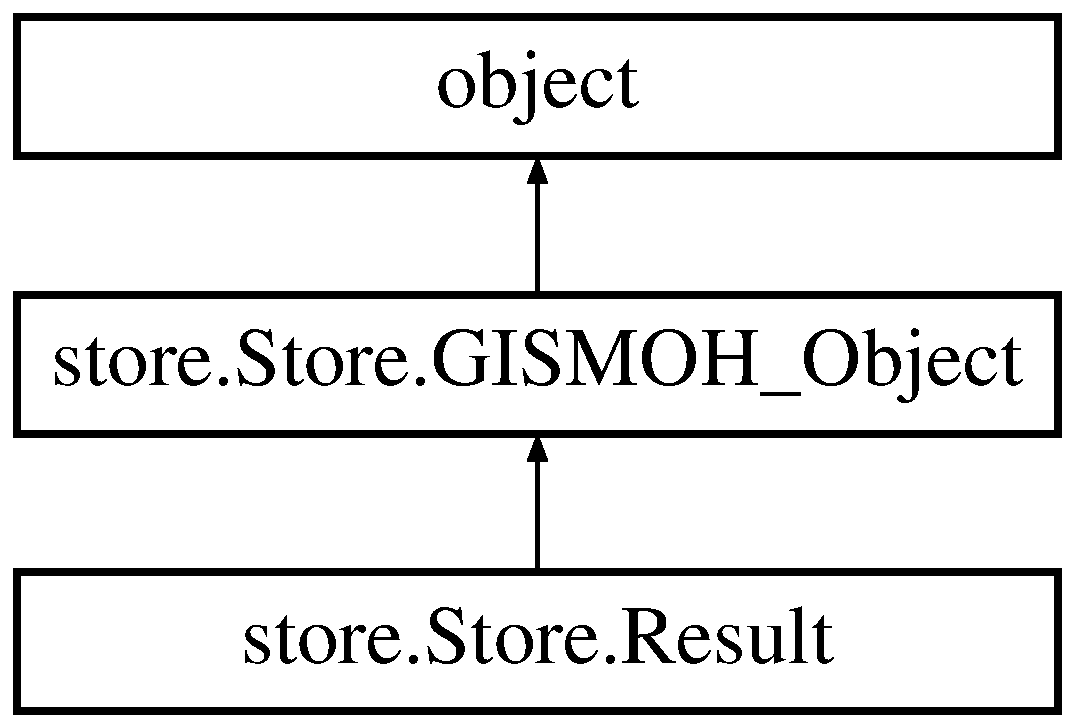
\includegraphics[height=3.000000cm]{classstore_1_1_store_1_1_result}
\end{center}
\end{figure}
\subsection*{Public Member Functions}
\begin{DoxyCompactItemize}
\item 
\hypertarget{classstore_1_1_store_1_1_result_a6f0d5d1bc4a54bf6d2633f1e3b21e8bd}{def {\bfseries get\-\_\-key}}\label{classstore_1_1_store_1_1_result_a6f0d5d1bc4a54bf6d2633f1e3b21e8bd}

\end{DoxyCompactItemize}
\subsection*{Static Public Attributes}
\begin{DoxyCompactItemize}
\item 
\hypertarget{classstore_1_1_store_1_1_result_a1f79dd282c1a466c756a81fd5dc6a4c2}{{\bfseries test\-\_\-type} = None}\label{classstore_1_1_store_1_1_result_a1f79dd282c1a466c756a81fd5dc6a4c2}

\item 
\hypertarget{classstore_1_1_store_1_1_result_a95b08efeba19e328bfa909ac27ee44c9}{{\bfseries result} = None}\label{classstore_1_1_store_1_1_result_a95b08efeba19e328bfa909ac27ee44c9}

\item 
\hypertarget{classstore_1_1_store_1_1_result_a3f42ca76b24b92b2f23dee79ca7b4b8f}{{\bfseries result\-\_\-type} = None}\label{classstore_1_1_store_1_1_result_a3f42ca76b24b92b2f23dee79ca7b4b8f}

\item 
\hypertarget{classstore_1_1_store_1_1_result_a77ef210d749a37d02140fbac6ed88326}{{\bfseries test\-\_\-date} = None}\label{classstore_1_1_store_1_1_result_a77ef210d749a37d02140fbac6ed88326}

\item 
\hypertarget{classstore_1_1_store_1_1_result_aa55b328d0989fa4b16dd8e17af62ba7f}{{\bfseries isolate\-\_\-id} = None}\label{classstore_1_1_store_1_1_result_aa55b328d0989fa4b16dd8e17af62ba7f}

\end{DoxyCompactItemize}


\subsection{Detailed Description}
Class that describes a test result such as an antibiogram. 

The documentation for this class was generated from the following file\-:\begin{DoxyCompactItemize}
\item 
store/Store.\-py\end{DoxyCompactItemize}

\hypertarget{classapplication_1_1_risk_and_positive_handler}{\section{application.\-Risk\-And\-Positive\-Handler Class Reference}
\label{classapplication_1_1_risk_and_positive_handler}\index{application.\-Risk\-And\-Positive\-Handler@{application.\-Risk\-And\-Positive\-Handler}}
}
Inheritance diagram for application.\-Risk\-And\-Positive\-Handler\-:\begin{figure}[H]
\begin{center}
\leavevmode
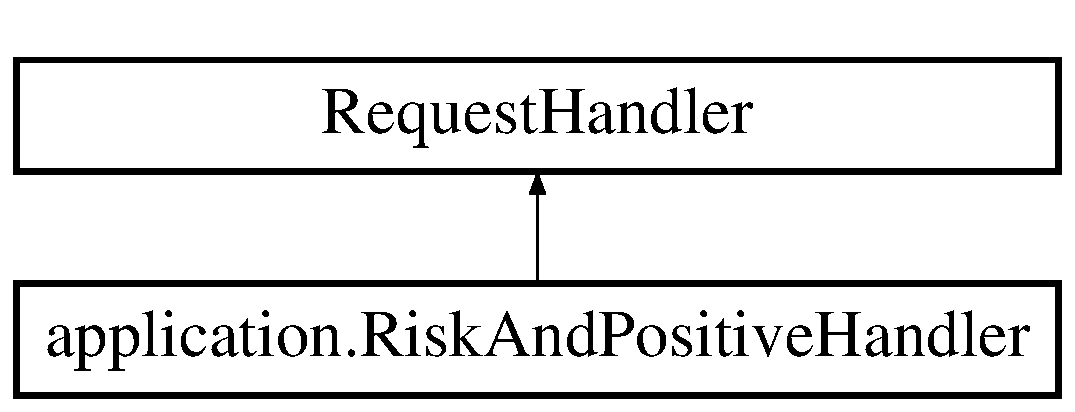
\includegraphics[height=2.000000cm]{classapplication_1_1_risk_and_positive_handler}
\end{center}
\end{figure}
\subsection*{Public Member Functions}
\begin{DoxyCompactItemize}
\item 
\hypertarget{classapplication_1_1_risk_and_positive_handler_a497de62ea0fd76c5f2c98961c05476f1}{def {\bfseries get}}\label{classapplication_1_1_risk_and_positive_handler_a497de62ea0fd76c5f2c98961c05476f1}

\end{DoxyCompactItemize}


The documentation for this class was generated from the following file\-:\begin{DoxyCompactItemize}
\item 
application.\-py\end{DoxyCompactItemize}

\hypertarget{classinterfaces_1_1scbu_1_1_s_c_b_u___importer}{\section{interfaces.\-scbu.\-S\-C\-B\-U\-\_\-\-Importer Class Reference}
\label{classinterfaces_1_1scbu_1_1_s_c_b_u___importer}\index{interfaces.\-scbu.\-S\-C\-B\-U\-\_\-\-Importer@{interfaces.\-scbu.\-S\-C\-B\-U\-\_\-\-Importer}}
}


Import data from the S\-C\-B\-U dataset.  


Inheritance diagram for interfaces.\-scbu.\-S\-C\-B\-U\-\_\-\-Importer\-:\begin{figure}[H]
\begin{center}
\leavevmode
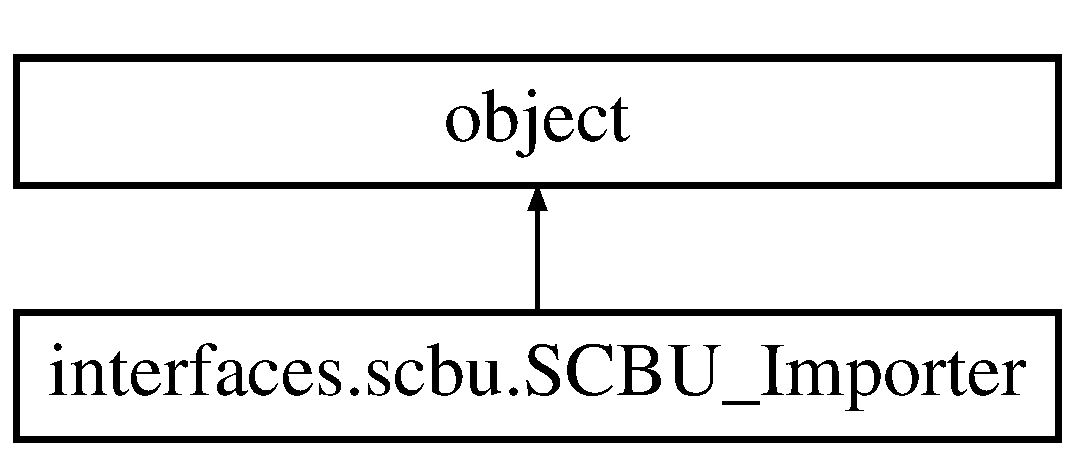
\includegraphics[height=2.000000cm]{classinterfaces_1_1scbu_1_1_s_c_b_u___importer}
\end{center}
\end{figure}
\subsection*{Public Member Functions}
\begin{DoxyCompactItemize}
\item 
\hypertarget{classinterfaces_1_1scbu_1_1_s_c_b_u___importer_a4310e98f8f35790aacf05b93ead2c82d}{def {\bfseries \-\_\-\-\_\-init\-\_\-\-\_\-}}\label{classinterfaces_1_1scbu_1_1_s_c_b_u___importer_a4310e98f8f35790aacf05b93ead2c82d}

\item 
\hypertarget{classinterfaces_1_1scbu_1_1_s_c_b_u___importer_a06971583e80184b2a9df31e9851ffc82}{def {\bfseries read\-\_\-admissions}}\label{classinterfaces_1_1scbu_1_1_s_c_b_u___importer_a06971583e80184b2a9df31e9851ffc82}

\item 
\hypertarget{classinterfaces_1_1scbu_1_1_s_c_b_u___importer_af33ca39f561a06a52cd587e69dc1c5fb}{def {\bfseries read\-\_\-isolates}}\label{classinterfaces_1_1scbu_1_1_s_c_b_u___importer_af33ca39f561a06a52cd587e69dc1c5fb}

\item 
\hypertarget{classinterfaces_1_1scbu_1_1_s_c_b_u___importer_a7c8ddb25c73b2ce5964dd8f3d66d1d4f}{def {\bfseries row\-\_\-reader}}\label{classinterfaces_1_1scbu_1_1_s_c_b_u___importer_a7c8ddb25c73b2ce5964dd8f3d66d1d4f}

\item 
\hypertarget{classinterfaces_1_1scbu_1_1_s_c_b_u___importer_aae60a9a7be72f16395ce06e97319a3b9}{def {\bfseries read\-\_\-patient}}\label{classinterfaces_1_1scbu_1_1_s_c_b_u___importer_aae60a9a7be72f16395ce06e97319a3b9}

\item 
\hypertarget{classinterfaces_1_1scbu_1_1_s_c_b_u___importer_a28452dce028c58a59319075970f2bf9b}{def {\bfseries read\-\_\-isolate}}\label{classinterfaces_1_1scbu_1_1_s_c_b_u___importer_a28452dce028c58a59319075970f2bf9b}

\end{DoxyCompactItemize}
\subsection*{Public Attributes}
\begin{DoxyCompactItemize}
\item 
\hypertarget{classinterfaces_1_1scbu_1_1_s_c_b_u___importer_af44236e3ec523c91419ffa313387270c}{{\bfseries store}}\label{classinterfaces_1_1scbu_1_1_s_c_b_u___importer_af44236e3ec523c91419ffa313387270c}

\end{DoxyCompactItemize}
\subsection*{Static Public Attributes}
\begin{DoxyCompactItemize}
\item 
\hypertarget{classinterfaces_1_1scbu_1_1_s_c_b_u___importer_a7b3c9ec1b884cde729ec0d82801b846b}{{\bfseries reader} = None}\label{classinterfaces_1_1scbu_1_1_s_c_b_u___importer_a7b3c9ec1b884cde729ec0d82801b846b}

\end{DoxyCompactItemize}


\subsection{Detailed Description}
Import data from the S\-C\-B\-U dataset. 

The documentation for this class was generated from the following file\-:\begin{DoxyCompactItemize}
\item 
interfaces/scbu.\-py\end{DoxyCompactItemize}

\hypertarget{classtests_1_1scbu__importer_1_1_s_c_b_u___tests}{\section{tests.\-scbu\-\_\-importer.\-S\-C\-B\-U\-\_\-\-Tests Class Reference}
\label{classtests_1_1scbu__importer_1_1_s_c_b_u___tests}\index{tests.\-scbu\-\_\-importer.\-S\-C\-B\-U\-\_\-\-Tests@{tests.\-scbu\-\_\-importer.\-S\-C\-B\-U\-\_\-\-Tests}}
}
Inheritance diagram for tests.\-scbu\-\_\-importer.\-S\-C\-B\-U\-\_\-\-Tests\-:\begin{figure}[H]
\begin{center}
\leavevmode
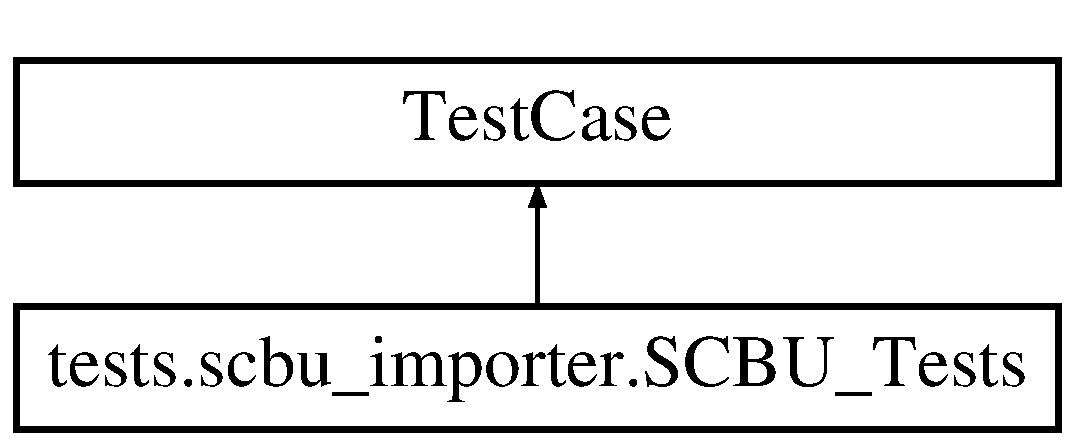
\includegraphics[height=2.000000cm]{classtests_1_1scbu__importer_1_1_s_c_b_u___tests}
\end{center}
\end{figure}
\subsection*{Public Member Functions}
\begin{DoxyCompactItemize}
\item 
\hypertarget{classtests_1_1scbu__importer_1_1_s_c_b_u___tests_ae8554d0a16d6e2c85e640527573d89f6}{def {\bfseries test\-\_\-create\-\_\-interface}}\label{classtests_1_1scbu__importer_1_1_s_c_b_u___tests_ae8554d0a16d6e2c85e640527573d89f6}

\item 
\hypertarget{classtests_1_1scbu__importer_1_1_s_c_b_u___tests_aa72ca14218b25daa974eae95a4b742c1}{def {\bfseries test\-\_\-do\-\_\-import}}\label{classtests_1_1scbu__importer_1_1_s_c_b_u___tests_aa72ca14218b25daa974eae95a4b742c1}

\item 
\hypertarget{classtests_1_1scbu__importer_1_1_s_c_b_u___tests_aaa6cb756780e5d15b4b05879c029553a}{def {\bfseries test\-\_\-get\-\_\-patient}}\label{classtests_1_1scbu__importer_1_1_s_c_b_u___tests_aaa6cb756780e5d15b4b05879c029553a}

\item 
\hypertarget{classtests_1_1scbu__importer_1_1_s_c_b_u___tests_a8951def68b8e0dff5185611260d14130}{def {\bfseries test\-\_\-get\-\_\-location}}\label{classtests_1_1scbu__importer_1_1_s_c_b_u___tests_a8951def68b8e0dff5185611260d14130}

\item 
\hypertarget{classtests_1_1scbu__importer_1_1_s_c_b_u___tests_a65015ae87467710ad7e0e60cb5cd9282}{def {\bfseries test\-\_\-get\-\_\-result}}\label{classtests_1_1scbu__importer_1_1_s_c_b_u___tests_a65015ae87467710ad7e0e60cb5cd9282}

\end{DoxyCompactItemize}


The documentation for this class was generated from the following file\-:\begin{DoxyCompactItemize}
\item 
tests/scbu\-\_\-importer.\-py\end{DoxyCompactItemize}

\hypertarget{classtests_1_1test__stores_1_1sqlite__test}{\section{tests.\-test\-\_\-stores.\-sqlite\-\_\-test Class Reference}
\label{classtests_1_1test__stores_1_1sqlite__test}\index{tests.\-test\-\_\-stores.\-sqlite\-\_\-test@{tests.\-test\-\_\-stores.\-sqlite\-\_\-test}}
}
Inheritance diagram for tests.\-test\-\_\-stores.\-sqlite\-\_\-test\-:\begin{figure}[H]
\begin{center}
\leavevmode
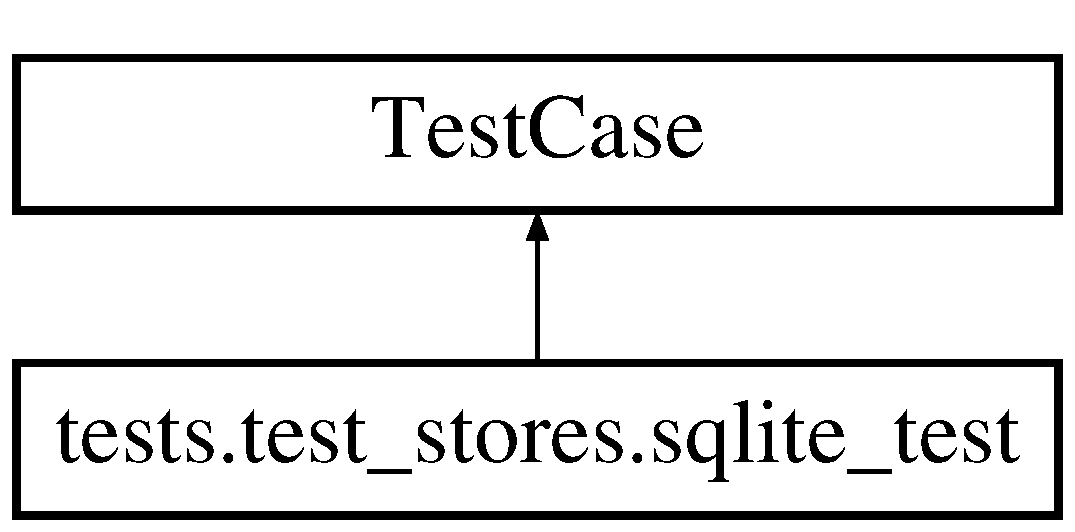
\includegraphics[height=2.000000cm]{classtests_1_1test__stores_1_1sqlite__test}
\end{center}
\end{figure}
\subsection*{Public Member Functions}
\begin{DoxyCompactItemize}
\item 
\hypertarget{classtests_1_1test__stores_1_1sqlite__test_ac7e870c7b3992aaebbe7b79c745da8fd}{def {\bfseries test\-\_\-connect}}\label{classtests_1_1test__stores_1_1sqlite__test_ac7e870c7b3992aaebbe7b79c745da8fd}

\item 
\hypertarget{classtests_1_1test__stores_1_1sqlite__test_a0c3eab179470d84e633656fa43d0a47c}{def {\bfseries test\-\_\-mapper}}\label{classtests_1_1test__stores_1_1sqlite__test_a0c3eab179470d84e633656fa43d0a47c}

\item 
\hypertarget{classtests_1_1test__stores_1_1sqlite__test_a089d774289e05ab810966484c380907b}{def {\bfseries test\-\_\-create\-\_\-query}}\label{classtests_1_1test__stores_1_1sqlite__test_a089d774289e05ab810966484c380907b}

\end{DoxyCompactItemize}


The documentation for this class was generated from the following file\-:\begin{DoxyCompactItemize}
\item 
tests/test\-\_\-stores.\-py\end{DoxyCompactItemize}

\hypertarget{classstore_1_1_store_1_1_s_q_lite_store}{\section{store.\-Store.\-S\-Q\-Lite\-Store Class Reference}
\label{classstore_1_1_store_1_1_s_q_lite_store}\index{store.\-Store.\-S\-Q\-Lite\-Store@{store.\-Store.\-S\-Q\-Lite\-Store}}
}
\subsection*{Public Member Functions}
\begin{DoxyCompactItemize}
\item 
\hypertarget{classstore_1_1_store_1_1_s_q_lite_store_a007e6b708dacb48c4d0b0ddaec7df28c}{def {\bfseries \-\_\-\-\_\-init\-\_\-\-\_\-}}\label{classstore_1_1_store_1_1_s_q_lite_store_a007e6b708dacb48c4d0b0ddaec7df28c}

\item 
\hypertarget{classstore_1_1_store_1_1_s_q_lite_store_a2c265207a658772856f9d322af5e4848}{def {\bfseries get}}\label{classstore_1_1_store_1_1_s_q_lite_store_a2c265207a658772856f9d322af5e4848}

\item 
\hypertarget{classstore_1_1_store_1_1_s_q_lite_store_a5c5bbac644cd2457d02be525ffbf6669}{def {\bfseries save}}\label{classstore_1_1_store_1_1_s_q_lite_store_a5c5bbac644cd2457d02be525ffbf6669}

\item 
\hypertarget{classstore_1_1_store_1_1_s_q_lite_store_a2d29ac35f67f1e29160ff8d7a6cf2d4e}{def \hyperlink{classstore_1_1_store_1_1_s_q_lite_store_a2d29ac35f67f1e29160ff8d7a6cf2d4e}{find}}\label{classstore_1_1_store_1_1_s_q_lite_store_a2d29ac35f67f1e29160ff8d7a6cf2d4e}

\begin{DoxyCompactList}\small\item\em find and item of type cls where \end{DoxyCompactList}\item 
\hypertarget{classstore_1_1_store_1_1_s_q_lite_store_a02f2b71123ddb656b9fc558229a7f530}{def {\bfseries create\-Insert\-Query}}\label{classstore_1_1_store_1_1_s_q_lite_store_a02f2b71123ddb656b9fc558229a7f530}

\end{DoxyCompactItemize}
\subsection*{Static Public Attributes}
\begin{DoxyCompactItemize}
\item 
\hypertarget{classstore_1_1_store_1_1_s_q_lite_store_a15742f03d65865e047de6cf63e1affbd}{{\bfseries db} = None}\label{classstore_1_1_store_1_1_s_q_lite_store_a15742f03d65865e047de6cf63e1affbd}

\end{DoxyCompactItemize}


The documentation for this class was generated from the following file\-:\begin{DoxyCompactItemize}
\item 
store/Store.\-py\end{DoxyCompactItemize}

%--- End generated contents ---

% Index
\newpage
\phantomsection
\addcontentsline{toc}{part}{Index}
\printindex

\end{document}
